\documentclass{sig-alternate}

\usepackage{graphicx}

\hyphenation{op-tical net-works semi-conduc-tor}
\usepackage{float}

\begin{document}

\title{Attack Surface Measurement on Android Applications}

\author{
  Kevin Campusano\\
  B. Thomas Golisano College of Computing and Information Sciences\\
  Rochester Institute of Technology\\
  Rochester, New York 14623\\
  Email: kac2375@rit.edu\\
  Advisor: Dr. Andy Meneely
}

\maketitle

\begin{abstract}

Mobile devices have seen an explosive increment in use and have become integral to our everyday lives. With processing power comparable to conventional desktop machines, these devices are capable of meeting our most common computing needs. To achieve this, smart devices access and manipulate sensitive information and this is why they represent a security risk. We propose using the concept of attack surface to create a metric to characterize the security of Android applications. In this study, we develop a methodology and tools for calculating the attack surface of Android applications and derive metrics from it. After that, we use data from real world, readily available Android applications to validate our proposed metrics. We also contribute with a set of programs to mine the Google Play Store for information regarding the applications and a list of all the Android framework API calls that constitute flow of data into and out of the applications.

\end{abstract}

\section{Introduction}

Mobile devices have seen an explosive increment in use during the past few years. With the advent of tablets, phones and other smart devices, computing has taken a new, more accessible and portable form and has become integral to our everyday lives now more than ever. With processing power comparable to conventional desktop machines, these devices are capable of meeting our most common computing needs. To achieve this, smart devices access and manipulate sensitive information such as location, calendars and emails. Indeed, smart devices provide a lot of convenience. However, due to the amount of sensitive information they manage, they also represent a security risk.

In this day and age only a handful of different mobile platforms hold the majority of the market share. Among those, Android has seen an outstanding growth in its install base and now holds a privileged position of more than half of smartphone users in the US \cite{_android_news}. Due in part to its popularity, the Android platform has been the target of multiple attacks \cite{vidas_all_2011}. Even though Android's application development framework and the operating system itself provide (although not perfect \cite{shabtai_google_2010}) many defense mechanisms \cite{burns2009mobile} \cite{enck2011study}, the responsibility to protect sensitive information ultimately falls to application developers as their applications are what interact directly with the users and their information.

With security being such an important concern, the need for it to be managed is imperative. For software security to be managed and subsequently improved, measuring it, as is the case with most quality attributes, is essential. To address this problem we propose the use of a measurement of applications' attack surface based on their call graph information \cite{Manadhata2011AnAttackSurfaceMetric}.

The attack surface is defined as all the different ways in which a malicious user can take advantage of a system and compromise its data. It can be thought as the "attackability" of a system. We can say then, that the smaller a system's attack surface is, the more secure it is \cite{Manadhata2011AnAttackSurfaceMetric}.

We propose using the concept of attack surface to create a metric to characterize the security of Android applications. To guide our efforts, we have the following research questions:

\begin{itemize}
  
\item \textbf{RQ1: Does the attack surface of Android applications affect their perceived security?} 

When developing metrics one key aspect of the work is to validate the metric. In other words, we need to find out whether the metric truly represents the property that it is trying to measure. To know if the attack surface of Android applications is useful for measuring their security we need to see if the metrics correspond to some sort of ground truth: something that we know reflects an application's security. We use user's security related complaints for this.

We discovered that there is a weak correlation between the size of the attack surface and the user's perceived security of Android apps. 

\item \textbf{RQ2: Does the attack surface of Android applications affect their rating?}

Another way to give credibility to the attack surface as a metric for Android application security is to find how high and low rated applications compare in terms of their attack surface. We also try to find a correlation between the metrics and the user ratings.

We discovered that the size of the attack surface of low rated applications is statistically smaller than that of high rated applications. We also discovered a weak correlation between the metrics and the ratings of the applications. We did see, however, that the majority of applications with bigger attack surface were rated between 4 and 4.5.

\end{itemize}

Past research in the area of Android application security has focused on enhancements to the application development framework's security aspects \cite{ongtang_semantically_2012}, application privilege \cite{bugiel2012towards} and inter-application communication \cite{chin_analyzing_2011}. There has been previous work on attack surface of android \cite{bartel_automatically_2012} that used call graph information of applications to identify permission gaps. Our approach proposes the use of call graph information to measure and characterize the attack surface and use this to observe the difference in security between various versions of studied applications.

\section{Android Application Development Platform Overview}

The Android platform provides developers with a rich application development framework that contains a varied collection of libraries for most common functionalities and for interaction with the device's physical components. This development framework provides a core set of building blocks that most Android applications are constructed with:

\subsection{Activities}

The most common of the framework's main building blocks. All applications that involve some sort of interaction with the user are composed of at least one Activity. Activities are what provide user interfaces for the applications. In a traditional sense, each activity would correspond to a “screen”, so to speak. They contain both graphical user interface definitions and code.

\subsection{Services}

Services embody operations that run in the background without any interaction with the user. Downloading a file or continuously keeping email synchronized are some examples of functionality that are typically implemented as services.

\subsection{Broadcast Receivers}

These are components that are responsible of receiving messages (i.e. Intents) from other applications or services that are intended to be handled for multiple applications. More often than not, a Broadcast Receiver's sole purpose is to relay the received messages to an Activity or Service that supports the particular operation specified in the Intent.

\subsection{Content Providers}

These are shared storage resources that can be accessed by multiple applications using their assigned URIs. These are used for both data persistence and information sharing between apps.

\subsection{Intents}

Android's inter process communication mechanisms are built around Intents. These are objects that encapsulate a message which typically contains a recipient, an operation and some data to work with. Intents can be sent both from the operating system and applications and can be handled by Activities, Services and Broadcast Receivers.

Depending on how the recipient for the operation described in the intent is specified, these can be of two types: Explicit and Implicit. Explicit Intents specify their recipient application while the Implicit ones describe their recipient as any application that meets certain criteria (i.e. that support the operation that the Intent represents). Implicit Intents rely on the Android platform to find a suitable application to handle it. The operating system also allows the user to select which application to handle such operations if multiple applications that support that functionality are installed in the device.

\section{Android Security Model Overview}

Android is in essence a linux based operating system build from the ground up with a focus on mobile devices and security as one of its main design goals. As such, there are security mechanisms put in place at the operating system level that affect how the users interact with their devices.

\subsection{The Market}

There are many different virtual markets from where users can obtain Android applications. The biggest one of these is the Google Play store. One of the core objectives of the Android platform is to keep it accessible both to developers and users. The process of getting applications in the store is simple and the cost is minimal. While this strategy is sound for ensuring the growth and relevance of the platform, it is not as sound for security purposes. Ill intentioned developers won't find much resistance in getting malicious applications into the Android market which will subsequently reach consumer devices and potentially compromise them and their users' data.

\subsection{Permissions}

Android's security model is permission based. This means that the concept of permissions plays an integral role in the security of the platform. These permissions are what control the applications' access to the user's personal data store in the device as well as access to any physical component on the device. Android permissions range from access to the user's contacts information to the ability to use of the camera installed in the device.

Prior to installing an application, the underlying operating system prompts the user with the permissions that the application about to be installed requires to function. The user has the option to accept or decline installing the application after (hopefully) carefully reviewing the permissions requested. These permissions are specified by the developers as part of the application's source files.

\subsection{Runtime}

At runtime, all the applications that are installed in the device are executed in isolation. The kernel provides a sandboxing mechanism that allows the applications to run separate to each other and to the rest of the system functions. In their sandbox, each application has its own set of resources that are not shared with any other running process. Each application runs in a different instance of the interpreter. 

This design prevents any application from accessing private data from the system and from other applications.

\subsection{Inter-application Communication}

Even though, by design, applications run in isolation in the Android platform, there are mechanisms for interprocess communication in place. In Android, interprocess communication is achieved by one of the basic building blocks of the Android application development framework: Intents. Intents are objects that can be instantiated by any application and the operating system itself and encapsulate a message that can be sent to other running processes. This message generally contains information for the receiver about what operation to perform, what data to work with or both.

When Intents are sent, they can be directed to a specific application or to any application that supports handling the particular action specified in the Intent. For example, an application that requires the camera may not directly use it but invoke the default camera application installed in the device. For this, the requesting application will create an Intent and configure it to be handled by the camera application. Likewise, the operating system could use Intents to notify a power saving application when the battery life has reached a certain threshold of consumption.

\section{Related Work}

There has been extensive work in the area of security in the Android platform. 

\subsection{Android Security}

Shabtai et al. \cite{shabtai_google_2010} performed a comprehensive security assessment of the Android platform. They evaluated all security concepts and mechanisms used in the platform. Both those that are inherited from the Linux kernel and new to the Android operating system itself. They identified potential weaknesses on the security mechanisms of the platform and offered several techniques that could be used to address these weaknesses. 

Gommerstadt et al. \cite{gommerstadt2012android} developed a model of the information flow in Android applications with a focus on the flow of private and sensitive data. They use previous studies on Android security as a base for their model and present two applications as case studies as a way for using their model to study the flow of information.

\subsection{Taxonomy of Android Attacks}

Vidas et al. \cite{vidas_all_2011} from the Carnegie Mellon University developed a taxonomy of all the known attacks that targeted the Android platform. The classification they proposed grouped the attack classes into two categories depending on the access that the attacker would need on the device: Attacks with physical access and attacks with no physical access.

\subsubsection{Attacks without physical access}

For these types of attacks, the attacker need not have physical access to the targeted device. Generally, these attacks consist on the attacker finding the way to execute malicious code on the device. In essence, this means that the attacker convinces the user to trust and run their code one way or the other. Once the malicious code is running on the targeted device, any vulnerability can be exploited to obtain privileged access and compromise the user's sensitive data or cause other manners of harm.

\textbf{Unprivileged Attacks}: Although the way that most attacks can maximize the damage they cause in a device is by obtaining elevated privileges, there is still fair amount of harm that can be done without breaking free from the Android security model. Still within their sandbox, with standard application permissions, malware can be dangerous. 

Some of the ways that seemingly benign applications can reach a user's device is by installing them directly from the Internet bypassing and ignoring any operating system warning as well as installing applications that request a large number of permissions at install time with dubious purposes. The Google Play Store as well as many other Android markets provide a web based interface that users can use to remotely install applications to their devices. If an attacker were to somehow hijack the user's session or authentication credentials, then they would have the ability to install any malicious application to the user's device and potentially compromise it. In addition to these methods, application repacking is a threat present in Android markets. Application repacking consists on the attacker downloading and decompiling existing popular applications, injecting malicious code into them and reuploading them to the market. Since these repacked applications are identical to their legitimate counterparts, users are tricked into installing them without a second thought and subsequently running malicious code on their device.

\textbf{Privileged Attacks}: Attacks consisting on obtaining elevated privileges and remotely executing code are based on many of the same techniques discussed earlier. The attacker somehow finds a way to get malicious code to execute on the targeted device, the difference is that this code's purpose is to perform a privilege escalation attack. Code that executes with elevated privilege in the device is outside the restrictions of all of the platform's security mechanisms and as such has a great potential of causing harm.

These kinds of remote exploitation attacks can also be achieved without the installation of malicious software in the target device. Vulnerabilities in common software that mobile devices use like web browsers or even the underlying Linux kernel can be exploited to run harmful code with high privilege.

Bugiel et al \cite{bugiel2012towards} explore the problem of developing a framework to protect the Android platform against two specific types of privilege escalation attacks: confused deputy and collusion attacks. They contribute with ways to improve the security of Android against these types of attacks.

\subsubsection{Attacks with physical access}

Of course, physical security is still a valid concern. This category describes the attacks that can be done when the attacker obtains physical access to the device.

\textbf{ADB enabled}: The Android Developer Bridge is a program that aids in the development and debugging of Android applications from a computer connected to a device. If an attacker gains physical access to a device where the Android Developer Bridge is enabled they can hook it up to a computer that has the Android developer tools installed and interact with the device. This can be done even if the device is obstructed with mechanisms such as lock screens. Via the ADB, the attacker is able to run untrusted code in the device and, as a consequence, compromise user information. Privilege escalation attacks can also be performed this same way by running the exploits from the ADB.

\textbf{ADB disabled}: If an attacker gains access to a device that is obstructed and in which the ADB is disabled, there are still options available to take advantage of it. The way to attack such a device is by booting the device in recovery mode using a forged recovery image. When booting from this image, the attacker has total control over the device and can run malicious code or gain elevated privileges.

\textbf{On unobstructed devices}: This is the best case scenario for the attacker. If the attacker gains physical access to an unattended device that is not obstructed in any way (e.g. no screen lock) then the effort needed to run malicious code in it is minimal. In this situation any of the previously discussed attack methods are available.

Based on their proposed taxonomy and the attacker's capabilities, Vidas et al. also designed a flowchart of how an attacker would approach a breach into an Android system. It can be seen in Figure \ref{fig:attackflow}.

\begin{figure}
  \centering
  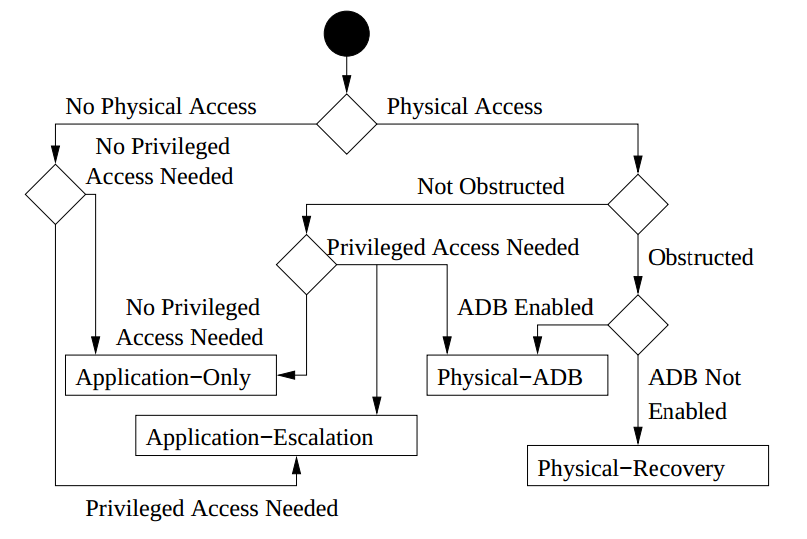
\includegraphics[scale=0.30]{figs/attackflow.png}
  \caption{Android attack flowchart developed by Vidas et al.}
  \label{fig:attackflow}
\end{figure}

\subsection{The Attack Surface}

As Manadhata and Wing \cite{Manadhata2011AnAttackSurfaceMetric} put it: "A system's attack surface is the subset of its resources that an attacker can use to attack the system." In their work Manadhata et al. \cite{Manadhata2011AnAttackSurfaceMetric} come up with a definition for a multi-dimensional metric for attack surfaces based on many factors. One particularly important is the count of Entry and Exit Points of the system under analysis. They develop a methodology for obtaining systems' Entry and Exit Points based on their call graph. Both static (compile-time) and dynamic (runtime) data is needed for a comprehensive call graph.

In subsequent work, Manadhata et al. \cite{manadhata_measuring_2006} \cite{manadhata2009report} use their developed methodology to measure and study the attack surface of industrial and open source software. In  \cite{manadhata_measuring_2006} they present a case study on two applications in the same domain. The authors apply the concepts explored in their previous work and put them to practice with two case studies. They use their multi-dimensional attack surface metric to compare the security attribute of two Unix FTP Daemons: ProFTPD and WuFTPD. This paper provides a real-world scenario in which an attack surface metric could be used to support software acquisition decisions by comparing the attack surface of two or more software alternatives.

In \cite{manadhata2009report} they present another case study, this time with an enterprise software written in Java: SAP. They implement their metric calculation methodology as an eclipse IDE plugin. In this case study, they present their metric as a complementary approach to general code quality assessments for software security.

\subsection{The Attack Surface in Android}

Previous work on attack surface of Android applications has focused on inter-application communication \cite{chin_analyzing_2011} and permission gaps \cite{bartel_automatically_2012}. Bartel et al. \cite{bartel_automatically_2012} focus on the "permission-gap” and uses that to define the attack surface in Android applications. They define this as the mismatch between the permissions that an application requests at installation-time and the ones that it actually uses. Their premise is that the bigger the difference between permissions quantity the larger the attack surface because there are more permissions requested but not needed. They develop a static analysis based method to extracting the call graph information of Android applications calculate their permission gap.

Chin et al. \cite{chin_analyzing_2011} explore another aspect of Android applications' security related to the attack surface: inter-application communication. They explain the risks that come with inter-application communication and present a tool they developed to analyze applications and detect vulnerabilities.

Our approach proposes the use of call graph information to measure and characterize the attack surface of Android applications.

\section{Concepts}

\subsection{Attack Surface Definition}

"A system's attack surface is the subset of its resources that an attacker can use to attack the system." \cite{Manadhata2011AnAttackSurfaceMetric}. Given this definition, it stands to reason that the most important aspects of a systems attack surface are the openings through which said system resources can be accessed and potentially exploited by an attacker. We call these openings Entry and Exit Points.

Figure \ref{fig:androidattacksurfacemodel} shows a model of how the attack surface works for Android applications in terms of the agents that applications interact with. In Android, there are four main entities that applications interact with (I.e. Data flows from and to): the network, the file system, the device hardware and the user. In the case of Android applications all this interaction takes place leveraging platform APIs that invoke Framework and Operating System functions.

\begin{figure}
  \centering
  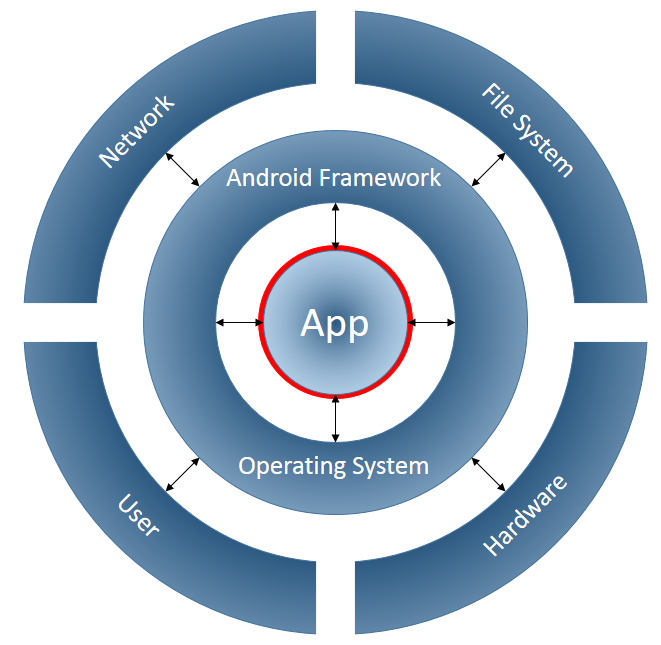
\includegraphics[scale=0.30]{figs/androidattacksurfacemodel.png}
  \caption{A model of how the attack surface works in Android. Through the framework and operating system layer, Android applications interact with the network, the file system, the hardware and the users.}
  \label{fig:androidattacksurfacemodel}
\end{figure}

With this concept of attack surface in mind, we define what we consider as Entry and Exit points for this study in the following sections.

\subsection{Entry Point Definition}

We define an Entry Point in an Android application as any method that represents an interaction between the application and an agent in the it's environment in which data is entering the application in order for it to work with or use that data in some way. This agent can be either the file system, the network, the hardware sensors, the user or the underlying operating system and framework.

Practically speaking, an Entry Point in the context of an Android application is any application-defined method that contains one or more calls to framework-defined Input Methods.

\subsection{Exit Point Definition}

We define an Exit Point in an Android application as any method that represents an interaction between the application and an agent in the application's environment in which data is exiting the app to it's environment. This agent can be either the file system, the network, the hardware sensors, the user or the underlying operating system and framework.

Practically speaking, an Exit Point in the context of an Android application is any application-defined method that contains one or more calls to framework-defined Output Methods.

\subsection{Android's Special Case of Entry and Exit Points}

Due to the Android framework's particular mechanisms in which it interacts with apps, we needed to expand the Entry and Exit Points practical definition to include certain callback methods. One of the Android framework’s interaction mechanisms with apps is through callbacks. Many events that happen in the device, the operating system and even other apps are communicated to the apps through callback methods that each app defines to respond or handle said events. A number of these callback methods constitute ways in which information enters and/or exits the applications and as such, we consider them as Entry and Exit points even though they may not adhere to the base practical definition of containing calls to Input or Output methods.

\section{Methodology}

\begin{figure*}
  \centering
  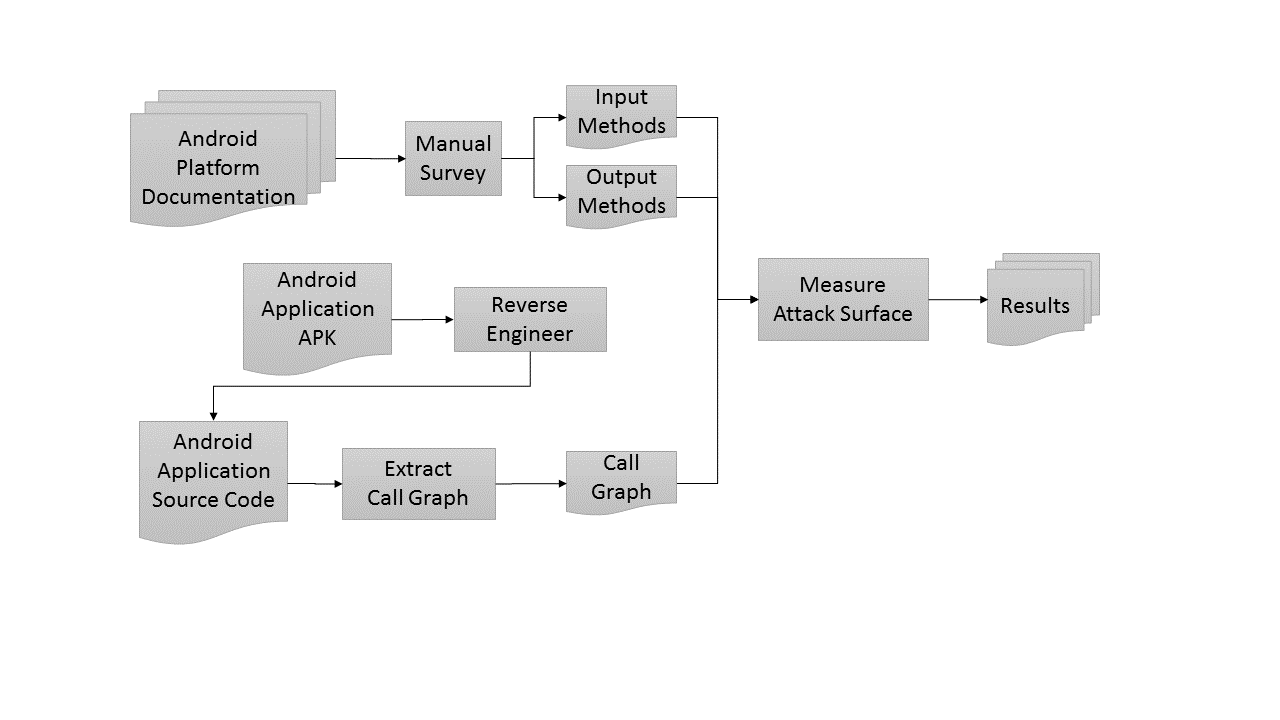
\includegraphics[scale=0.45]{figs/methodology.png}
  \caption{Overview of the attack Surface measurement methodology}
  \label{fig:methodology}
\end{figure*}

Our study's main objective is to develop a method for obtaining the attack surface of Android applications and validate whether the metrics derived from it truly represent an application's security.

The following sections describe the approach taken in this project to obtain the necessary data and address our research questions. Figure \ref{fig:methodology} shows an overview of the methodology.

\subsection{Data Collection}

We obtain all the data necessary to answer our research questions from one single source: The Google Play Store. From here, we extract three distinct bodies of information: 

\begin{enumerate}
\item Application meta data.
\item The user reviews of the applications.
\item The installation package (APK) of every application.
\end{enumerate}

\subsubsection{Downloading Google Play Store Application Meta Data}

We build a scraper using \cite{scrapy} and based on the one used by \cite{googleplay_scraper}. This program's purpose is to crawl through the Google Play Store and download the meta data of all the applications that it encounters. This data includes the applications' rating, URL from within the store, number of downloads, number of reviews, among others.

Using this method, we are able to download meta data for 38,302 unique applications from the Google Play Store and store all this data in a relational data base.

\subsubsection{Downloading Google Play Store Application Reviews}

We build another program that downloads the user reviews of all the applications scraped in the previous step.

This method has its limitations due to Google's policy for scripted automatic requests. We have to work around this by strategically delaying execution between subsequent requests. This poses a considerable cost of time to the whole downloading process but it is unavoidable since, without that delay, Google will block all requests coming from that same location for as much as 24 hours. Each request downloads one page of reviews which contain at most 40 reviews.

In spite of this limitation we obtain a total of 2,243,319 unique reviews coming from 18,802 applications and store them in our database.

\subsubsection{Downloading Google Play Store Application APKs}

We build yet another program that uses the scraped applications' URLs to download all the installation packages.

Similarly to the previous step of downloading the applications' reviews, we need to put a delay in the execution of our program between each request. This considerably increases the time it takes to download the APKs for our complete data set.

We are able to obtain the APKs for 26,648 of the scraped applications.

\subsection{Data Processing}

Once we have the applications' installation packages (APK) we use an in-house developed program that extracts the call graph of all the APKs. This program is built using other third party tools. Specifically:

\begin{enumerate}

\item \textbf{jar}. We use this Java Development Kit utility to extract the "classes.dex" file from an APK. This file contains the source code for all the classes that the application packaged in a given APK contains.

\item \textbf{dex2jar}. This tool is used to turn the .dex file into a .jar file. jar files are the main form of distributable packages in the Java Development Kit.

\item \textbf{java-callgraph}. This tool provides the functionality to generate the call graph of a given .jar through static analysis. Its output contains both dependencies between classes and methods. It shows how the classes relate to each other in terms of the members that they call on each other. It also shows the relations among methods in terms of what methods call each other. Four our purposes, we only use the method invocation related info since that is all we need to generate the call graph.

We save all the call graphs of the downloaded applications' installation packages as text files using the program discussed earlier.

At this point, we now have applications meta data, user reviews for those applications and the call graphs.

\end{enumerate}

\subsection{Calculating the Attack Surface Metrics}

One of our study's main objectives is to develop a method for measuring the attack surface of Android applications based on Entry Points and Exit Points obtained from their call graph information. This is the point when we come to realize that vision. By definition, Entry Points are the functions, methods or procedures through which data flows into the system. Similarly, Exit points are those through which data flows out of the system. Simply put, Entry Points are methods that contain calls to APIs for data input (i.e. Input Methods) and Exit Points are methods that contain calls to APIs for data output (i.e. Output Methods). The basic process for measuring the attack surface in terms of Entry Points and Exit Points involves obtaining the applications call graph from the source code and identifying all the Entry and Exit points in the call graph.

In order to be able to identify Entry and Exit points in a call graph, we need to know which are the Input and Output methods of a particular environment. In our case, that environment is Android.

\subsubsection{Discovering Android Framework's Input and Output Methods}

As described earlier, our definition for Entry and Exit Points depends heavily on Input and Output Methods. We define an Input Method as any framework-defined method in which information is flowing into the application. Again, the source of this information can be either the file system, the network, the hardware, the user or the underlying operating system and framework. We define Output methods similarly: an Output Method is any framework-defined method in which information is flowing out of the application.

To identify the Android framework’s Input and Output methods we studied the API guides and reference contained in the documentation available in the Android Developers site \cite{android_developers} and developed a list of 364 Input Methods and 304 Output Methods.

Both our definition for Entry and Exit Points and the model we developed for how the attack surface works for Android applications (Figure \ref{fig:androidattacksurfacemodel}) were instrumental in our process of discovering input and output methods when reviewing the Android framework's documentation. They provided a point of reference on which to base our decisions for which API methods to include in our lists of input and output methods. Particularly important to this process was the notion that applications interact with five main agents in their environment: the user, file system, the hardware, the network and the framework and operating system itself. We will organize the discussion of our decision process in detail using these as categories.

\textbf{Interacting with the user:} All the methods that allowed the user to provide information to and consume information from the application were included. A traditional method for users to directly enter and receive information into the system is through the graphical user interface. The Android framework provides an event driven model for developing GUIs. For example, when the user taps a button, let's say to submit a form, an event in the system is generated that invokes an event handler (or listener) method that is defined in the application's code. The event handler method would then proceed to obtain a reference to one or more objects that represent the text boxes that are present in the current screen (i.e. Activity) and invoke accessors and mutators to get and set values in the current state of those widgets. Accessors would allow the application code to obtain, for example, the text that the user entered in those text boxes. Mutators would allow the application code to set the text of those text boxes with the results of some operation that was performed. This kind of design is typical in many GUI frameworks and libraries and are classical examples of Input and Output Methods. 

All of the accessors that provide the application access to the values of the various widgets were included into the list of Input Methods and all of the mutators that set the values of the various widgets' were included into the list of Output Methods. Some examples for Input Methods in this category are methods that get the text from a text box widget, or a selection from a selection box widget. Some examples for Output Methods in this category are methods that set the text from a text box widget, or a selection for a selection box widget. Specific GUI related methods are further discussed in the following section about notable examples of Input and Output methods.

\textbf{Interacting with the file system:} There are many facilities that are provided by the Android framework for interaction with files. A couple of very important aspects of mobile application development is localization and internationalization. The Android framework provides support for those in the form of a rich resource API. Many components in an Android application, from simple pieces of text to entire GUI layouts are managed as resources. These resources are stored in files that are distributed with the applications (inside the APKs) but separate from the actual executable. There are many APIs for accessing and loading these resources. We included these methods into out Input Method list. 

There is also a rich stream based API for working with files that is part of the Java Standard Libraries and is available for Android application development. We included the methods for opening and reading in the list of Input Methods and the ones for writing and creating files in the Output Method list. All of the methods that opened streams or took data coming from a stream and made it available for an application to use were considered as Input Methods. All of the methods that open streams and write application data to a stream were included as Output Methods.

\textbf{Interacting with the hardware:} Android powered devices come with a number of sensors and hardware components like movement sensors, GPS, cameras, bluetooth transceivers and USB ports that application developers can leverage to enhance their users' experience. Of course, the Android framework provides a set of APIs for interacting with these sensors and hardware components. As they constitute a source of external data, we included all methods that read data from these components into our Input Method list. The ones that write data to these components we considered Output Methods. 

There are also a number of methods in the API available for interacting with these hardware components that operate with an event driven model. That meas that there are methods defined in the application code that are invoked by the framework and receive data from the sensors and hardware components as parameters. These event handlers constitute Input Methods because they are a point through which external data enters the application.

\textbf{Interacting with the network:} Much of the API that the Android framework provides for network interaction is stream based. So the reasoning discussed in the previous paragraph about interactions with the file system not only applies to files but also to resources that are accessed through the network. Another series of API methods work on an event driven model. We included these methods as well based on that same reasoning explained in the last paragraph about hardware interactions.

\textbf{Interacting with the framework and OS:} Android applications don't live in isolation. The Android framework was designed with communication between applications and the system in mind and the mechanisms that are in place for that constitute a part of the attack surface of Android applications. Such mechanisms work mainly through an event driven model which has been discussed in earlier. The Intent class is a key part of this as it contains the bundle of data that travels from application to application and from and to the system. There are many event handlers that the framework invokes when out-of-application communication is taking place that receive Intents as input parameters. We have included such event handlers in our lists. Accessors for the Intent class itself have not been included in the list. Our reasoning behind it is that the external data is already in the application's domain when an event handler that receives an Intent as a parameter is invoked by the system.

At the other end of the spectrum of out-of-application interaction are a set of methods that allow applications to invoke other applications or system components as opposed to being invoked themselves. Again, Intents play an essential role in this interactions where the invoking application needs to instantiate an Intent object and load it with the data that needs to be transferred to the receiving end. We chose to include the methods that actually send out the bundle of information represented by the Intent (i.e. startActivity and related methods).

The Android framework also provides facilities for interacting with system wide functionality like alarms, accounts, policies, notifications, backup and other data exposed through, among others, ContentProviders. We took these APIs into consideration and included the methods for interacting with these in our Input and Output Methods lists.

In summary: for Input Methods, all the API methods that provided functionality to get data into applications from their environment were included in the list. For Output Methods, all the API methods that provided functionality to put data out of applications to their environment were included in the list. The Appendix contains the lists we developed and used in this study.

\begin{figure}
  \centering
  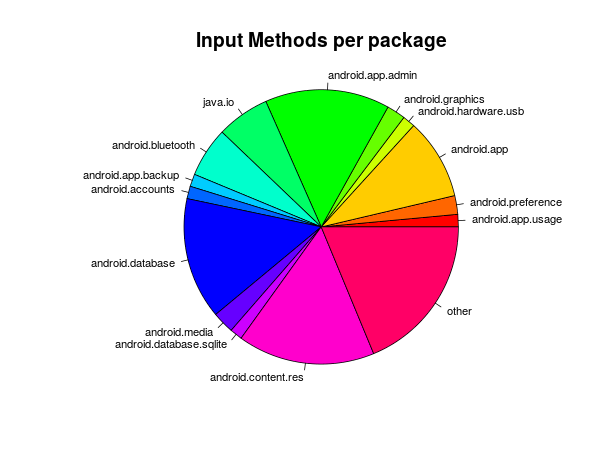
\includegraphics[scale=0.40]{figs/input_methods_per_package.png}
  \caption{Proportion of Input Methods per component in the Android Framework.}
  \label{fig:input_methods_per_package}
\end{figure}

\begin{figure}
  \centering
  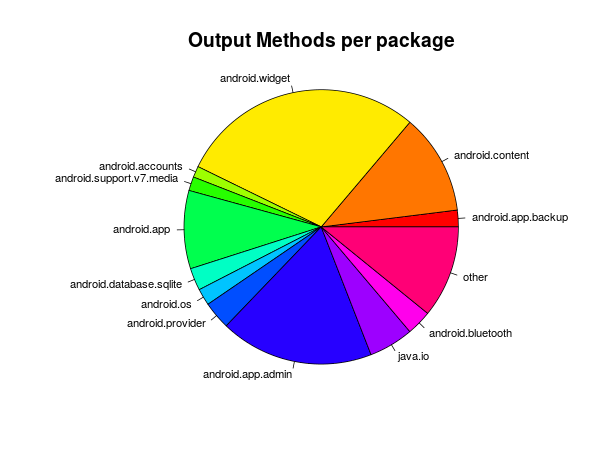
\includegraphics[scale=0.40]{figs/output_methods_per_package.png}
  \caption{Proportion of Output Methods per component in the Android Framework.}
  \label{fig:output_methods_per_package}
\end{figure}

Figures \ref{fig:input_methods_per_package} and \ref{fig:output_methods_per_package} shows the proportional amount of methods that each android component contributes to our lists of Input and Output Methods. The appendix contains tables that present this same data for every package that for which there are methods in the lists. The pie charts only show those packages for which there are 1\% or more methods in their respective lists.

\subsubsection{Input Methods Notable Examples}

The discovered Input Method list is very diverse. There are methods like "android.app.Activity.onCreate" which is an application-defined method that is implemented in classes that inherit from the "android.app.Activity" class (one of the main building blocks of Android apps that represents a "screen" in an app). This method serves as a callback that the framework invokes when the Activity in question is being created and passes it a bundle of external data encapsulated in an Intent. Recall that an Intent encapsulates a message which contains data that can come from within the app, other apps or from the system. This "onCreate" callback is one of those special cases described in the previous section. It is identified as an Input Method during our Android framework documentation survey but practically it acts as an Entry Point.

There are also instances that exemplify a more traditional notion of Input Method such as methods as "android.widget.\-EditText.\-getText", "android.widget.\-CheckBox.\-isChecked" and "android.widget.\-CalendarView.\-getDate". These methods represent basic mechanisms through which the Android framework supports direct user interaction through the Graphical User Interface. Widgets such as EditTexts and CheckBoxes represent ways in which the user can enter information into the apps.

The Android framework provides a robust external resource management API ideal for localization, internationalization and even separation of concerns by storing XML files separate from the application's implementation. These files contain many resources from specific single point values like an integer or string or boolean to complete GUI templates and animation definitions. This API provides a number of methods for loading these resources into the application. There are many methods such as "android.\-content.\-res.\-Resources.\-getInteger" or "android.\-content.\-res.\-Resources.\-getBoolean" that given a resource identification number, return single pieces of information. Methods like "android.\-content.\-res.\-Resources.\-getLayout", "android.\-content.\-res.\-Resources.\-getConfiguration", "android.\-content.\-res.\-Resources.\-getAnimation" exemplify more complex data structures stored in these resource files and retrieved through the resources API. Even though these resource files are packaged inside the applications we consider these Entry Points as well because they represent data that is flowing into the application’s execution context and more importantly, can be tampered with.

The complete list of the Android framework Input Methods that we used for our study can be found in the appendix.

\subsubsection{Output Methods Notable Examples}

The "android.app.\-Activity.\-startActivity" method provides very important functionality. This single method is responsible for allowing applications to communicate within themselves and with other applications in the device. "startActivity" purpose is to initiate other Activities. Its uses can range from opening anothe screen in the application to invoking other applications such as an email client or the camera application. All forms of "startActivity" receive an Intent as a parameter which, as discussed before, contains information that will be passed from the application to the component (I.e. Activity) that this method is invoking. There are other methods similar to "startActivity" that are provid similar functionality. Such as: "startActivityForResult", "startActivityFromChild", "startActivityFromFragment", etc. "android.content.Context.sendBroadcast" is a method similar in purpose to "startActivity" but geared towards interacting with Broadcast Receivers instead of general Activities.

The Android framework also provides methods for interacting with internal databases like "android.\-database.\-sqlite.\-SQLiteDatabase.\-insert" or "android.\-database.\-sqlite.\-SQLite\-Database.\-update".

Other more traditional Output Methods that we found were methods that provided support for writing data to the file system like "android.\-content.\-Context\-Wrapper.\-open\-File\-Output". There are also methods that are not particular to the Android framework that serve similar purposes such as "java.\-io.\-OutputStream.\-write". These are methods defined in the Java Standard Library and are also available for Android application development. 

Methods that were used to present information to the users were also taken into consideration. Some examples are: "android.\-widget.\-Toast.\-show", "android.\-widget.\-Edit\-Text.\-set\-Text", "android.\-widget.\-TextView.\-set\-Text".

We also included many methods that dealt with network communication. For example, the Android framework provides a set of APIs for interacting with the Bluetooth trans\-ceivers in the devices. Such as: "android.\-bluetooth.\-Bluetooth\-Gatt.\-begin\-Reliable\-Write", "android.\-bluetooth.\-Bluetooth\-Socket.\-get\-Output\-Stream", "android.\-bluetooth.\-Bluetooth\-Adapter.\-enable", "android.\-bluetooth.\-Bluetooth\-Gatt\-Server.\-send\-Response".

The complete list of the Android framework Output Methods that we used for our study can be found in the appendix.

\subsubsection{The Edge Black List}

When generating the call graph from the APKs we noticed that the tools (i.e. java-callgraph \cite{java_callgraph}) generate entries for methods and classes that are defined in other Android libraries and not in the actual application's source code. This introduces unwanted noise to our attack surface metric calculation process. 

To work around this inaccuracy we decide to develop an Edge Black List. This black list contains a list of all the edges that appear repeated in multiple applications. Each edge represents a call from one method to another. Our attack surface metrics calculation process treats those black list edges specially when analyzing each application's call graph and calculating the metrics. Every black list node encountered by the attack surface metrics calculation process is collapsed into the packages the calls involved in that edge belong to. For example, a call graph like the one in Figure \ref{fig:callgraph_sample_full} will be collapsed to one like Figure \ref{fig:callgraph_sample_collapsed} if the following edges are part of the black list:

\begin{enumerate}
\item p1.c1.m1 -> p1.c1.m2
\item p1.c1.m2 -> p2.c2.m1
\item p1.c1.m2 -> p2.c2.m2
\item p2.c2.m1 -> p2.c2.m2
\end{enumerate}

\begin{figure}
  \centering
  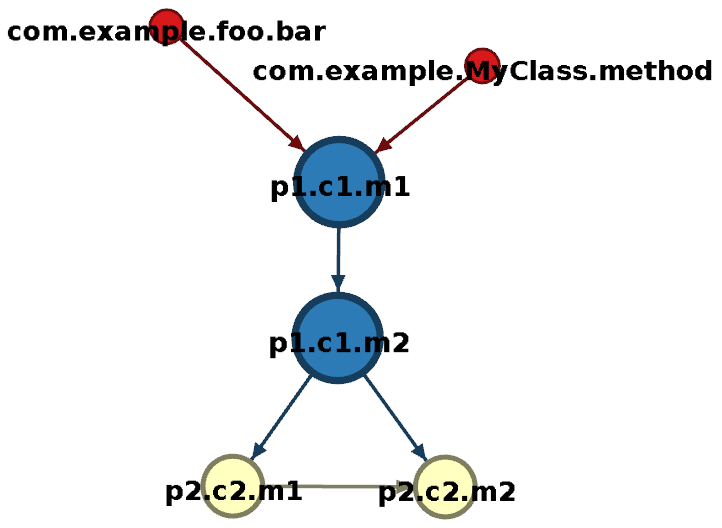
\includegraphics[scale=0.30]{figs/callgraph_sample_full.png}
  \caption{Call graph with edges in black list.}
  \label{fig:callgraph_sample_full}
\end{figure}

\begin{figure}
  \centering
  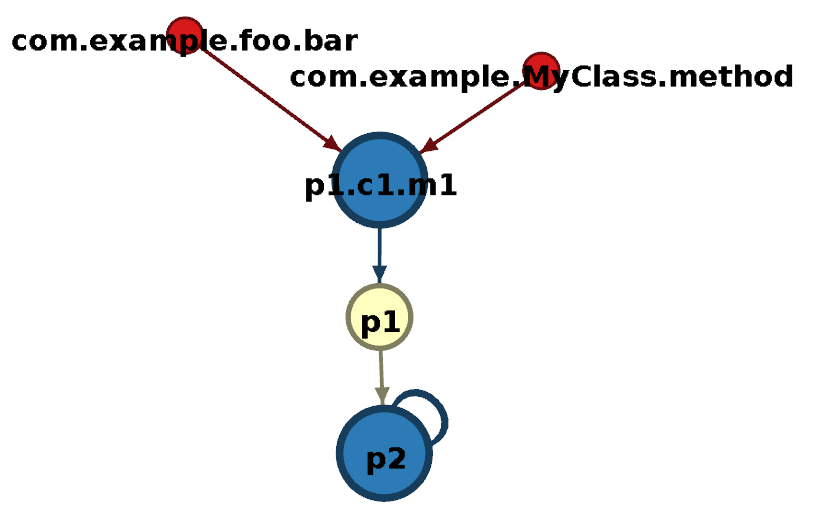
\includegraphics[scale=0.30]{figs/callgraph_sample_collapsed.png}
  \caption{Call graph with edges in black list that have been collapsed.}
  \label{fig:callgraph_sample_collapsed}
\end{figure}

In this example, nodes p2.c2.m1 and p2.c2.m2 have been collapsed into a single p2 node and the p1.c1.m2 node has been substituted for a p1 node. Notice how, even though the edge p1.c1.m1 -> p1.c1.m2 is in the black list, the node p1.c1.m1 stays in the call graph and is not collapsed into its corresponding package node. This happens because the p1.c1.m1 node is part of at least one edge that is not in the black list. In other words, p1.c1.m1 is called by methods defined in the actual applications source code. In this example the nodes com.example.foo.bar and com.\-example.\-MyClass.\-method represent methods defined in the application's source code, i.e. not in the black list.

To develop the Edge Black List for Android applications we generated the call graph of 250 applications chosen from the top applications in each category of the Google Play Store and found out the repeated edges. Edges that appeared in at least 10 of the applications were added to the black list.

The complete black list of edges of the Android framework that we used for our study can be found in \cite{attack_surface_meter}.

\subsubsection{Attack Surface Metrics Calculation}

Now, with a list of all the Input and Output Methods in the Android framework as well as an Android Application Edge Black List we have all the knowledge we need to successfully calculate the attack surface of Android applications.

To achieve this, we use the call graph files generated in the previously discussed step. With a program we developed that uses the Attack Surface Meter library \cite{attack_surface_meter} that we also developed we take the information in those call graph files and compute various attack surface metrics for each application. The calculated metrics are then saved into a relational data base. Our library provides functionality for calculating multiple metrics but we focus on two: Number of Entry Points and Exit Points. These two are the basis for measuring the size of attack surfaces.

During this phase of calculating the attack surface metrics we find out that call graph files bigger than a certain size take too much time to process so we decide to scale back the process and only use files smaller than 10.0 MB.

At this point, our data set consists of meta data, user reviews and the attack surface metrics of over 9000 applications.

\section{Results}

The following section goes into detail of our motivation, approach and findings related to both of our research questions. 

\subsection{RQ1: Is the attack surface of Android applications related to their perceived quality?}

\textbf{Motivation:} When developing metrics one key aspect of the work is to validate the metric. In other words, we need to find out whether the metric truly represents the property that it is trying to measure. To know if the attack surface of Android applications is useful for measuring their security we need to see if the metrics correspond to some sort of ground truth: something that we know reflects an application's security. We use user's security related complaints for this.

\textbf{Approach:} To try to answer this research question we need to know if the attack surface of the applications has any relation to their perceived security.

To discover the perceived security of an application, we count the number of reviews that contain complaints about security. The higher the number, the less secure the application is according to its users. We measure an application's perceived security by the number of user reviews that contain any of the words in a previously defined list that are deemed to reflect a user's negative experience with the application in terms of its security. We developed this list of words by manually reviewing a random sample of over two hundred reviews and identifying words that the users used to express security concerns with the applications. This is the list of words we discovered and used: 

\begin{itemize}
\item unsafe
\item glitch
\item rooted
\item permission
\item unlock
\item crash
\item scam
\item privacy
\item risk
\item pop
\end{itemize}

Words like unsafe, permission, risk, scam, privacy and pop (as in pup up) are directly related to security and we included them because we found instances in where the reviewers used these to express concern. Others like glitch, crash are widely used and reflect the general perception of quality of the application and refer to events that can have security related implications. The words root and unlock refer to methods that serve for users to gain elevated privileges in the devices and can potentially lead to security issues.

To determine whether a particular user review actually contained one of the aforementioned words we used the Natural Language Processing capabilities built into PostgreSQL which uses the stems of the words for comparison. In a nutshell, this process extracts the stem of all the words in the user review and compares each of those stems with the stems of the words in the list. If there is a match, that review is counted as a security complaint.

Figure \ref{fig:perceivedsecurity} shows a histogram of the distribution of the perceived security metric of the applications in our data set. Here we can see that the value of the metric decreases as the number of applications increases. We can also see that the vast majority of applications have very little (close to zero) reviews with security complaints. This means that in our data set, not many applications have high number of security complaints and most of them have close to 0 reviews with security complaints.

\begin{figure}
  \centering
  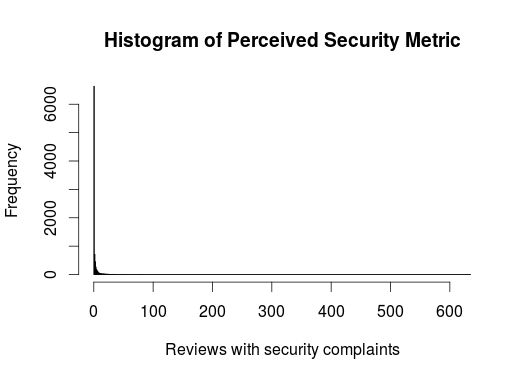
\includegraphics[scale=0.50]{figs/histogram_per_sec.png}
  \caption{The perceived security metric's distribution in our data set.}
  \label{fig:perceivedsecurity}
\end{figure}

For illustration purposes, we zoom in into the histogram and produce Figure \ref{fig:perceivedsecuritylimit50}. This histogram only shows the distribution of the values that are between 1 and 50. I.e. the applications that have between 1 and 50 reviews with security complaints. We can still see the same trend that the vast majority of applications have a small (between 0 and 20) number of reviews with security complaints compared with a limited number of outliers.

\begin{figure}
  \centering
  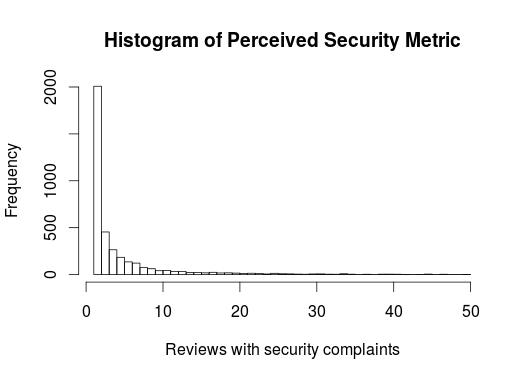
\includegraphics[scale=0.50]{figs/histogram_per_sec_limit_50.png}
  \caption{The distribution of the perceived security metric for values between 1 and 50.}
  \label{fig:perceivedsecuritylimit50}
\end{figure}

Our data set now contains a set of three values for each application: 1) the Number of Entry Points metric, 2) the Number of Exit Points metric and 3) a value that represents that application's perceived security which is the count of complaints that are related to security in the user reviews of that application. Let's call this last one the application's Perceived Security Metric.

Figures \ref{fig:entrypoints} and \ref{fig:exitpoints} show the distribution of the Entry Points and Exit Points metric in our data set. We can observe that the majority of applications have between 0 and 500 Entry Points and 0 and 200 Exit Points.

\begin{figure}
  \centering
  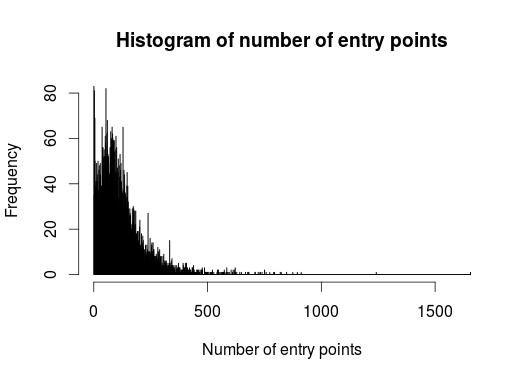
\includegraphics[scale=0.50]{figs/histogram_entry_points.png}
  \caption{The number of entry point metric's distribution in our data set.}
  \label{fig:entrypoints}
\end{figure}

\begin{figure}
  \centering
  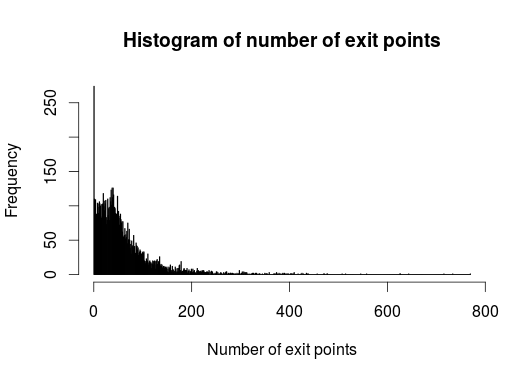
\includegraphics[scale=0.50]{figs/histogram_exit_points.png}
  \caption{The number of exit point metric's distribution in our data set.}
  \label{fig:exitpoints}
\end{figure}

With this data we then calculate the correlation coefficient of the applications' Perceived Security Metric and each of our two attack surface metrics: the Number of Entry Points and the Number of Exit Points.

% \ref{tab:result_rq1}
\textbf{Results:} Table 1 shows our results. We discovered that there is a positive but weak correlation between the size of the attack surface and the user's perceived security of Android applications. Given these results, we cannot conclude that the attack surface has some significant effect in the applications' security as perceived by the users. At least with our sample.

\begin{table}
\centering

\label{tab:result_rq1}

\begin{tabular}{|l|l|l|}
\hline
\textbf{Metric} & \textbf{Correlation} & \textbf{p-value}\\ 
\hline
Entry Points & 0.07719178 & < 0.05 \\
Exit Points & 0.06544354 & < 0.05 \\
\hline
\end{tabular}

\caption{Correlation between the size of the attack surface and the applications' perceived security.}

\end{table}

For further detail, we include Figures \ref{fig:entrypoints_seccomplaints} and \ref{fig:exitpoints_seccomplaints} that show the relation between the Entry and Exit Points metric and the Perceived Security metric (I.e. Number of security complaints.) These scatterplots show us a graphical representation of the values of our three metrics in the applications in our data set.

\begin{figure}
  \centering
  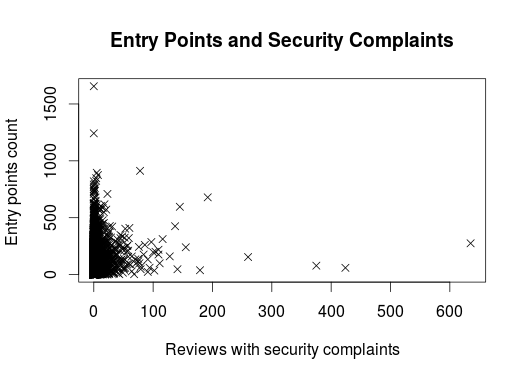
\includegraphics[scale=0.50]{figs/entry_points_sec_complaints.png}
  \caption{Relation between Entry Points and the Perceived Security of the applications in our data set.}
  \label{fig:entrypoints_seccomplaints}
\end{figure}

\begin{figure}
  \centering
  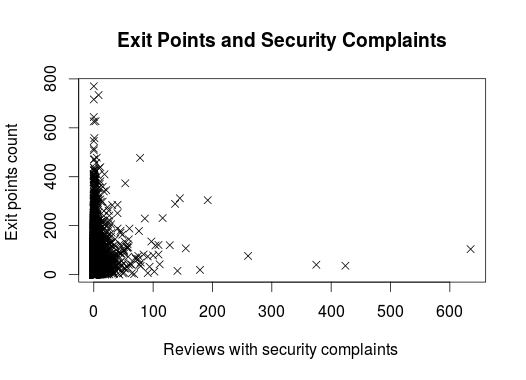
\includegraphics[scale=0.50]{figs/exit_points_sec_complaints.png}
  \caption{Relation between Exit Points and the Perceived Security of the applications in our data set.}  
  \label{fig:exitpoints_seccomplaints}
\end{figure}

\subsection{RQ2: Does the attack surface of Android applications affect their rating?}

\textbf{Motivation:} Another way to give credibility to the attack surface as a metric is to investigate what sort of relation it may have with the success of applications. Parting from the assumption that insecure applications will be rated lower than secure applications, we see if there's a statistical difference in the attack surface of low and high rated applications.

\textbf{Approach:} To answer our second research question we calculate the statistical difference in the attack surface of high vs low rated applications.

The first step of this process involves separating the applications in our data set in two groups: high rated apps and low rated apps. As part of the meta data that we mined from the applications in the Google PLay Store, we have each application's rating. This rating is represented as a number of "stars" between one and five and are given by the users. We decide to use a rating of "4 stars" as our threshold. Applications rated less than 4 stars were put in the group of low rated applications and those with a rating of 4 stars or higher were put in the high rated group.

We then used the Mann-Whitney Wilcoxon test to see if there was statistical difference between the Entry Points and Exit Points metrics of the two groups of applications. The Mann-Whitney Wilcoxon is a test that doesn't assume a normal distribution on the data and compares the statistical medians of two groups.

Another method that we can use to gain insight into a possible relation between the attack surface metrics and the success and quality of Android applications is testing for correlation. We can test to see if there is any correlation between the attack surface metrics and the rating of the applications.

% \ref{tab:result_rq2}
\textbf{Results:} Table 2 shows our results. We also include the box plots of these metrics in Figures \ref{fig:boxplot_entry_points} and \ref{fig:boxplot_exit_points} to graphically illustrate the difference between their values for high and low rated applications. We discovered that the size of the attack surface of low rated applications is statistically smaller than that of high rated applications. This difference is very small however. To put these results in perspective, for the applications in our data set, the average value for the Number of Entry Points metric is approximately 118 and our test results show that lower rated applications have approximately 8 fewer Entry Points than high rated applications. That is a difference of approximately 6 percent. In a similar way, the average value for the Number of Exit Points metric is approximately 61 for our sample and our test results show that lower rated applications have approximately 6 fewer Exit Points than high rated applications. That is a difference of approximately 9 percent.

These results could mean that applications with a bigger feature set have ultimately more points of interaction (i.e. Entry and Exit Points) and such applications are the ones that turn out to be more useful to users and, consequently, higher rated.

\begin{table}
  \centering

  \label{tab:result_rq2}

  \begin{tabular}{|l|l|l|l|}
  \hline
  \textbf{Metric} & \textbf{Difference} & \textbf{p-value} & \textbf{Avg. in sample}\\ 
  \hline
  Entry Points & 8.00001 & < 0.05 & 118.3 \\
  Exit Points & 6.000004 & < 0.05  & 61.7 \\
  \hline
  \end{tabular}

  \caption{Difference in the attack surface of high and low rated applications.}
\end{table}

\begin{figure}
  \centering
  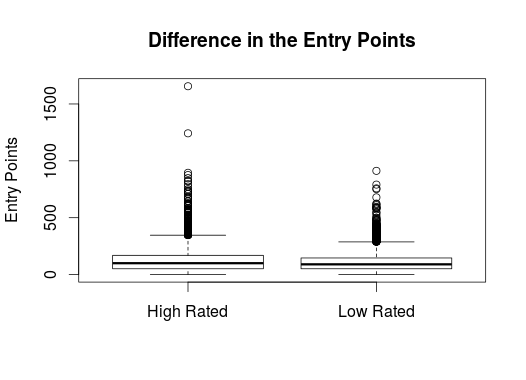
\includegraphics[scale=0.50]{figs/boxplot_entry_points.png}
  \caption{Difference in the Entry Points of high and low rated applications.}
  \label{fig:boxplot_entry_points}
\end{figure}

\begin{figure}
  \centering
  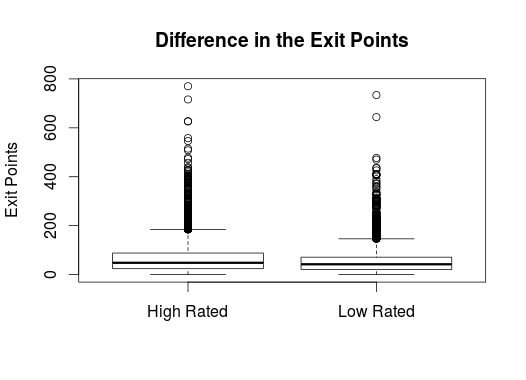
\includegraphics[scale=0.50]{figs/boxplot_exit_points.png}
  \caption{Difference in the Exit Points of high and low rated applications.}  
  \label{fig:boxplot_exit_points}
\end{figure}

%\ref{tab:result_rq2_2}
Table 3 shows the results we obtained for the correlation coefficients of Entry and Exit Points to user rating. For further detail, we include Figures \ref{fig:entry_points_user_rating} and \ref{fig:exit_points_user_rating} that show the values for the Entry and Exit Points metric for the applications in our data set for each user rating group. We can see here that the applications closer to the range of 4.0 to 4.5 in User Rating are the ones that have a higher count of Entry and Exit Points. Statistically however, the correlation is not strong so we can't conclude that the attack surface metrics we evaluate have any bearing in the rating of the applications.

\begin{table}
  \centering

  \label{tab:result_rq2_2}

  \begin{tabular}{|l|l|l|}
  \hline
  \textbf{Metric} & \textbf{Correlation} & \textbf{p-value}\\ 
  \hline
  Entry Points & 0.09993487 & < 0.05 \\
  Exit Points & 0.1049763 & < 0.05 \\
  \hline
  \end{tabular}

  \caption{Correlation between the size of the attack surface and the applications' user rating.}
\end{table}

\begin{figure}
  \centering
  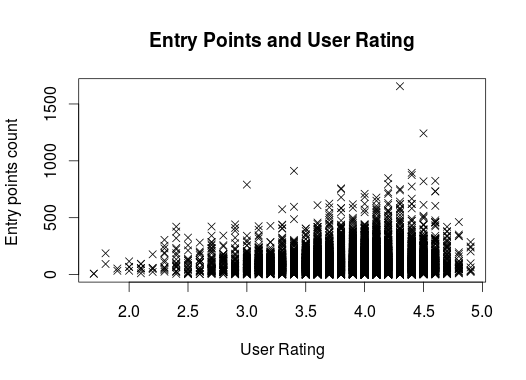
\includegraphics[scale=0.50]{figs/entry_point_user_rating.png}
  \caption{Relation between Entry Points and the User Rating of the applications in our data set.}
  \label{fig:entry_points_user_rating}
\end{figure}

\begin{figure}
  \centering
  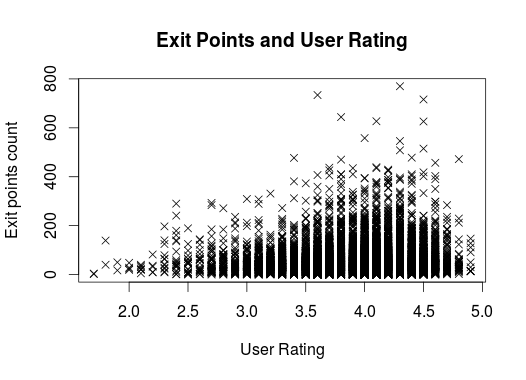
\includegraphics[scale=0.50]{figs/exit_point_user_rating.png}
  \caption{Relation between Exit Points and the User Rating of the applications in our data set.}  
  \label{fig:exit_points_user_rating}
\end{figure}

\section{Threats To Validity}

In this section we discuss any threats to the validity of our study that we acknowledge and how we dealt with them.

\subsection{Internal Validity}

The tools and libraries that we used and built in this project may include faults that could potentially invalidate our results. We reduced this threat however by thoroughly testing using an automated unit and integration test suite for the libraries and tools we built. The third party tools we used for reverse engineering applications were tested using a sample Android application we built so that we could validate the results.

To measure the perceived security of Android applications we counted the number of reviews that contained a specific list of words for each application. It is possible that we did not identified all the words that users use to express security related concerns and as a result, we were not able to identify all the reviews with security complaints. However, doing so would have required to manually go through hundreds of thousands of reviews and this is simply out of the scope of this study. For our current purposes, our method of manually reading a subset of the reviews to come up with a list of words and then automatically identifying the reviews with security complaints is appropriate.

\subsection{External Validity}

Even though we used a random sample and were able to collect a data set of more than 9000 applications, it may be difficult to generalize our results since they could not represent the vast population that is the applications available in the Google Play Store. Also, we could only use free applications for this study so we are not able to conclude anything about paid applications.

\section{Conclusion and Future Work}

This research project's main objectives were to develop a methodology for calculating the attack surface of Android applications and validate whether the metrics derived from it truly represent an application's security.

We have contributed to the body of knowledge of security with a methodology (accompanied with a set of open source programs, libraries and data) for calculating the attack surface of Android applications. Another important contribution has been the list of the Input and Output methods in the Android framework. This list is instrumental for the calculation of the attack surface and can prove very useful in other academic or industrial applications as well. We also contribute with a sizable data set containing information about tens of thousands of Android applications as well as a group of programs for mining Android applications' information from the Google Play Store.

Although with the analysis of our data set we did not obtain conclusive results, the notion of using attack surface derived metrics to measure the security of Android applications has not been invalidated altogether. There's still more work to be done in this area.

We saw from our results that, although correlations coefficients were low, we find promising the fact that the correlation is positive. Which means that the size of the attack surface and the security problems of Android applications grow together.

Further study is warranted with a bigger set of data that more accurately represents the entire population. Maybe another interesting path to pursue is using other information to compare the metrics against that is more accurate and trustworthy than user reviews. Users not always care about security or can't really identify when an application is doing something potentially insecure. 

Another place where there's room for further development is on the list of security complaints words we developed. More effort could be put into refining and expanding this list to make it comprehensive enough to capture more accurately the users complaints about security.

Finally, there are other metrics in addition to the ones we explored that can be derived from the attack surface. These metrics could prove to be more representative of the security of the Android environment in particular or software systems in general.

\bibliographystyle{IEEEtran}
\bibliography{capstone}

\onecolumn

\section{Appendix}

\subsection{Android Framework Input Method List}

This is the list of input methods that we found in API version 22 of the Android framework.

\begin{itemize}
  
\item android.content.ContentResolver.query
\item java.io.InputStream.read
\item android.animation.AnimatorInflater.loadAnimator
\item android.animation.AnimatorInflater.loadStateListAnimator
\item android.view.MenuInflater.inflate
\item android.content.res.Resources.getStringArray
\item android.content.res.Resources.getQuantityString
\item android.content.res.Resources.getBoolean
\item android.content.res.Resources.getColor
\item android.content.res.Resources.getDimension
\item android.content.res.Resources.getInteger
\item android.content.res.Resources.getIntArray
\item android.content.res.Resources.obtainTypedArray
\item android.content.res.Resources.getAnimation
\item android.content.res.Resources.getAssets
\item android.content.res.Resources.getBoolean
\item android.content.res.Resources.getColor
\item android.content.res.Resources.getColorStateList
\item android.content.res.Resources.getConfiguration
\item android.content.res.Resources.getDimension
\item android.content.res.Resources.getDimensionPixelOffset
\item android.content.res.Resources.getDimensionPixelSize
\item android.content.res.Resources.getDisplayMetrics
\item android.content.res.Resources.getDrawable
\item android.content.res.Resources.getDrawable
\item android.content.res.Resources.getDrawableForDensity
\item android.content.res.Resources.getDrawableForDensity
\item android.content.res.Resources.getFraction
\item android.content.res.Resources.getIdentifier
\item android.content.res.Resources.getIntArray
\item android.content.res.Resources.getInteger
\item android.content.res.Resources.getLayout
\item android.content.res.Resources.getMovie
\item android.content.res.Resources.getQuantityString
\item android.content.res.Resources.getQuantityString
\item android.content.res.Resources.getQuantityText
\item android.content.res.Resources.getResourceEntryName
\item android.content.res.Resources.getResourceName
\item android.content.res.Resources.getResourcePackageName
\item android.content.res.Resources.getResourceTypeName
\item android.content.res.Resources.getString
\item android.content.res.Resources.getStringArray
\item android.content.res.Resources.getSystem
\item android.content.res.Resources.getText
\item android.content.res.Resources.getTextArray
\item android.content.res.Resources.getValue
\item android.content.res.Resources.getValueForDensity
\item android.content.res.Resources.getXml
\item android.widget.EditText.getText
\item android.widget.CheckBox.isChecked
\item android.widget.RadioButton.isChecked
\item android.widget.ToggleButton.isChecked
\item android.widget.Switch.isChecked
\item android.widget.TimePicker.getCurrentHour
\item android.widget.TimePicker.getCurrentMinute
\item android.widget.DatePicker.getMonth
\item android.widget.DatePicker.getYear
\item android.widget.DatePicker.getDayOfMonth
\item android.widget.ArrayAdapter<T>.createFromResource
\item android.preference.PreferenceFragment.addPreferencesFromResource
\item android.preference.PreferenceFragment.loadHeadersFromResource
\item android.preference.Preference.persistBoolean
\item android.preference.Preference.persistFloat
\item android.preference.Preference.persistLong
\item android.preference.Preference.persistString
\item android.view.animation.AnimationUtils.loadAnimation
\item android.view.animation.AnimationUtils.loadInterpolator
\item android.view.animation.AnimationUtils.loadLayoutAnimation
\item android.view.View.setBackgroundResource
\item android.media.MediaPlayer.create
\item android.media.MediaPlayer.prepare
\item android.media.MediaPlayer.prepareAsync
\item android.media.MediaRecorder.start
\item android.media.JetPlayer.loadJetFile
\item android.media.JetPlayer.play
\item android.hardware.Camera.takePicture
\item android.hardware.Camera.startPreview
\item android.media.MediaRecorder.prepare
\item android.location.LocationManager.requestLocationUpdates
\item android.bluetooth.BluetoothServerSocket.accept
\item android.bluetooth.BluetoothSocket.getInputStream
\item android.nfc.tech.MifareUltralight.transceive
\item android.nfc.cardemulation.HostApduService.processCommandApdu
\item java.net.ServerSocket.accept
\item javax.net.ssl.SSLServerSocket.accept
\item java.net.Socket.getInputStream
\item javax.net.ssl.SSLSocket.getInputStream
\item android.hardware.usb.UsbManager.openAccessory
\item android.hardware.usb.UsbManager.openDevice
\item android.hardware.usb.UsbDeviceConnection.requestWait
\item android.hardware.usb.UsbRequest.queue
\item android.net.sip.SipAudioCall.answerCall
\item android.content.ClipboardManager.getPrimaryClip
\item android.content.ClipboardManager.getText
\item android.content.SharedPreferences.getAll
\item android.content.SharedPreferences.getBoolean
\item android.content.SharedPreferences.getFloat
\item android.content.SharedPreferences.getInt
\item android.content.SharedPreferences.getLong
\item android.content.SharedPreferences.getString
\item android.content.SharedPreferences.getStringSet
\item android.database.sqlite.SQLiteDatabase.execSQL
\item android.database.sqlite.SQLiteDatabase.query
\item android.database.sqlite.SQLiteDatabase.rawQuery
\item android.database.sqlite.SQLiteDatabase.rawQueryWithFactory
\item android.webkit.WebView.loadUrl
\item java.io.FileInputStream.read
\item java.io.DataInputStream.read
\item java.io.DataInputStream.readBoolean
\item java.io.DataInputStream.readByte
\item java.io.DataInputStream.readChar
\item java.io.DataInputStream.readDouble
\item java.io.DataInputStream.readFloat
\item java.io.DataInputStream.readFully
\item java.io.DataInputStream.readInt
\item java.io.DataInputStream.readLine
\item java.io.DataInputStream.readLong
\item java.io.DataInputStream.readShort
\item java.io.DataInputStream.readUTF
\item java.io.DataInputStream.readUnsignedByte
\item android.widget.AbsListView.getCheckedItemCount
\item android.widget.AbsListView.getCheckedItemIds
\item android.widget.AbsListView.getCheckedItemPosition
\item android.widget.AbsListView.getCheckedItemPositions
\item android.widget.AdapterView<T>.getSelectedItem
\item android.widget.AdapterView<T>.getSelectedItemId
\item android.widget.AdapterView<T>.getSelectedItemPosition
\item android.widget.AdapterViewAnimator.setInAnimation
\item android.widget.AdapterViewAnimator.setOutAnimation
\item android.widget.AdapterViewAnimator.getSelectedItem
\item android.widget.AdapterViewAnimator.getSelectedItemId
\item android.widget.AdapterViewAnimator.getSelectedItemPosition
\item android.widget.AdapterViewFlipper.getSelectedItem
\item android.widget.AdapterViewFlipper.getSelectedItemId
\item android.widget.AdapterViewFlipper.getSelectedItemPosition
\item android.widget.CalendarView.getDate
\item android.widget.CheckBox.isChecked
\item android.widget.CheckedTextView.isChecked
\item android.widget.CompoundButton.isChecked
\item android.widget.EditText.getText
\item android.widget.ExpandableListView.getSelectedId
\item android.widget.ExpandableListView.getSelectedPosition
\item android.widget.ImageButton.setImageResource
\item android.widget.ImageButton.setImageURI
\item android.widget.ImageSwitcher.setImageResource
\item android.widget.ImageSwitcher.setImageURI
\item android.widget.ImageView.setImageResource
\item android.widget.ImageView.setImageURI
\item android.widget.AutoCompleteTextView.getText
\item android.widget.MultiAutoCompleteTextView.getText
\item android.widget.NumberPicker.getValue
\item android.widget.RadioButton.isChecked
\item android.widget.RatingBar.getRating
\item android.widget.SearchView.getQuery
\item android.widget.SeekBar.getProgress
\item android.widget.ProgressBar.getProgress
\item android.widget.AbsSeekBar.getProgress
\item android.widget.Spinner.getSelectedItem
\item android.widget.Spinner.getSelectedItemId
\item android.widget.Spinner.getSelectedItemPosition
\item android.widget.StackView.setInAnimation
\item android.widget.StackView.setOutAnimation
\item android.widget.StackView.getSelectedItem
\item android.widget.StackView.getSelectedItemId
\item android.widget.StackView.getSelectedItemPosition
\item android.widget.Switch.isChecked
\item android.widget.TimePicker.getCurrentHour
\item android.widget.TimePicker.getCurrentMinute
\item android.widget.ToggleButton.isChecked
\item android.widget.VideoView.setVideoPath
\item android.widget.VideoView.setVideoURI
\item android.widget.ViewAnimator.setInAnimation
\item android.widget.ViewAnimator.setOutAnimation
\item android.widget.ViewSwitcher.setInAnimation
\item android.widget.ViewSwitcher.setOutAnimation
\item android.widget.ZoomButton.setImageResource
\item android.widget.ZoomButton.setImageURI
\item android.accounts.AccountManager.getAccounts
\item android.accounts.AccountManager.getAccountsByType
\item android.accounts.AccountManager.getAccountsByTypeAndFeatures
\item android.accounts.AccountManager.getAccountsByTypeForPackage
\item android.app.ActionBar.setCustomView
\item android.app.ActionBar.setIcon
\item android.app.ActionBar.setLogo
\item android.app.ActionBar.setSubtitle
\item android.app.ActionBar.setTitle
\item android.app.AlarmManager.getNextAlarmClock
\item android.app.DownloadManager.openDownloadedFile
\item android.app.WallpaperManager.setResource
\item android.app.WallpaperManager.setStream
\item android.app.admin.DevicePolicyManager.getAccountTypesWithManagementDisabled
\item android.app.admin.DevicePolicyManager.getActiveAdmins
\item android.app.admin.DevicePolicyManager.getApplicationRestrictions
\item android.app.admin.DevicePolicyManager.getAutoTimeRequired
\item android.app.admin.DevicePolicyManager.getCameraDisabled
\item android.app.admin.DevicePolicyManager.getCrossProfileCallerIdDisabled
\item android.app.admin.DevicePolicyManager.getCrossProfileWidgetProviders
\item android.app.admin.DevicePolicyManager.getCurrentFailedPasswordAttempts
\item android.app.admin.DevicePolicyManager.getInstalledCaCerts
\item android.app.admin.DevicePolicyManager.getKeyguardDisabledFeatures
\item android.app.admin.DevicePolicyManager.getMaximumFailedPasswordsForWipe
\item android.app.admin.DevicePolicyManager.getMaximumTimeToLock
\item android.app.admin.DevicePolicyManager.getPasswordExpiration
\item android.app.admin.DevicePolicyManager.getPasswordExpirationTimeout
\item android.app.admin.DevicePolicyManager.getPasswordHistoryLength
\item android.app.admin.DevicePolicyManager.getPasswordMaximumLength
\item android.app.admin.DevicePolicyManager.getPasswordMinimumLength
\item android.app.admin.DevicePolicyManager.getPasswordMinimumLetters
\item android.app.admin.DevicePolicyManager.getPasswordMinimumLowerCase
\item android.app.admin.DevicePolicyManager.getPasswordMinimumNonLetter
\item android.app.admin.DevicePolicyManager.getPasswordMinimumNumeric
\item android.app.admin.DevicePolicyManager.getPasswordMinimumSymbols
\item android.app.admin.DevicePolicyManager.getPasswordMinimumUpperCase
\item android.app.admin.DevicePolicyManager.getPasswordQuality
\item android.app.admin.DevicePolicyManager.getPermittedAccessibilityServices
\item android.app.admin.DevicePolicyManager.getPermittedInputMethods
\item android.app.admin.DevicePolicyManager.getScreenCaptureDisabled
\item android.app.admin.DevicePolicyManager.getStorageEncryption
\item android.app.admin.DevicePolicyManager.getStorageEncryptionStatus
\item android.app.backup.BackupDataInputStream.read
\item android.app.job.JobScheduler.getAllPendingJobs
\item android.app.usage.UsageStatsManager.queryAndAggregateUsageStats
\item android.app.usage.UsageStatsManager.queryConfigurations
\item android.app.usage.UsageStatsManager.queryEvents
\item android.app.usage.UsageStatsManager.queryUsageStats
\item android.bluetooth.BluetoothA2dp.getConnectedDevices
\item android.bluetooth.BluetoothA2dp.getDevicesMatchingConnectionStates
\item android.bluetooth.BluetoothAdapter.getAddress
\item android.bluetooth.BluetoothAdapter.getScanMode
\item android.bluetooth.BluetoothAdapter.getState
\item android.bluetooth.BluetoothGatt.getConnectedDevices
\item android.bluetooth.BluetoothGatt.readCharacteristic
\item android.bluetooth.BluetoothGatt.readDescriptor
\item android.bluetooth.BluetoothHeadset.startVoiceRecognition
\item android.bluetooth.BluetoothSocket.getInputStream
\item android.bluetooth.le.BluetoothLeScanner.startScan
\item android.content.AsyncQueryHandler.startQuery
\item android.content.ContentProviderClient.query
\item android.content.ContentProviderClient.openFile
\item android.content.ContentProviderClient.openAssetFile
\item android.content.res.ObbScanner.getObbInfo
\item android.database.AbstractCursor.getBlob
\item android.database.AbstractCursor.getColumnCount
\item android.database.AbstractCursor.getColumnIndex
\item android.database.AbstractCursor.getColumnIndexOrThrow
\item android.database.AbstractCursor.getColumnName
\item android.database.AbstractCursor.getColumnNames
\item android.database.AbstractCursor.getCount
\item android.database.AbstractCursor.getDouble
\item android.database.AbstractCursor.getExtras
\item android.database.AbstractCursor.getFloat
\item android.database.AbstractCursor.getInt
\item android.database.AbstractCursor.getLong
\item android.database.AbstractCursor.getNotificationUri
\item android.database.AbstractCursor.getPosition
\item android.database.AbstractCursor.getShort
\item android.database.AbstractCursor.getString
\item android.database.AbstractCursor.getType
\item android.database.DatabaseUtils.queryNumEntries
\item android.database.DatabaseUtils.stringForQuery
\item android.database.DatabaseUtils.blobFileDescriptorForQuery
\item android.database.DatabaseUtils.createDbFromSqlStatements
\item android.database.DatabaseUtils.cursorDoubleToContentValues
\item android.database.DatabaseUtils.cursorDoubleToContentValuesIfPresent
\item android.database.DatabaseUtils.cursorDoubleToCursorValues
\item android.database.DatabaseUtils.cursorFloatToContentValuesIfPresent
\item android.database.DatabaseUtils.cursorIntToContentValues
\item android.database.DatabaseUtils.cursorIntToContentValues
\item android.database.DatabaseUtils.cursorIntToContentValuesIfPresent
\item android.database.DatabaseUtils.cursorLongToContentValues
\item android.database.DatabaseUtils.cursorLongToContentValues
\item android.database.DatabaseUtils.cursorLongToContentValuesIfPresent
\item android.database.DatabaseUtils.cursorRowToContentValues
\item android.database.DatabaseUtils.cursorShortToContentValuesIfPresent
\item android.database.DatabaseUtils.cursorStringToContentValues
\item android.database.DatabaseUtils.cursorStringToContentValues
\item android.database.DatabaseUtils.cursorStringToContentValuesIfPresent
\item android.database.DatabaseUtils.cursorStringToInsertHelper
\item android.database.DatabaseUtils.longForQuery
\item android.database.DatabaseUtils.stringForQuery
\item android.gesture.GestureLibraries.fromFile
\item android.gesture.GestureLibraries.fromPrivateFile
\item android.gesture.GestureLibraries.fromRawResource
\item android.graphics.Movie.decodeFile
\item android.graphics.Movie.decodeStream
\item android.graphics.BitmapFactory.decodeFile
\item android.graphics.BitmapFactory.decodeFileDescriptor
\item android.graphics.BitmapFactory.decodeResource
\item android.graphics.BitmapFactory.decodeStream
\item android.mtp.MtpDevice.getObject
\item android.net.LocalSocket.getInputStream
\item android.net.LocalServerSocket.accept
\item android.net.http.AndroidHttpClient.execute
\item android.net.nsd.NsdManager.discoverServices
\item android.os.DropBoxManager.getNextEntry
\item android.os.MemoryFile.getInputStream
\item android.provider.Browser.getAllBookmarks
\item android.provider.Browser.getAllVisitedUrls
\item android.speech.SpeechRecognizer.startListening
\item dalvik.system.DexFile.entries
\item dalvik.system.DexFile.loadClass
\item dalvik.system.DexFile.loadDex
\item android.util.Base64InputStream.read
\item java.io.FileReader.read
\item java.io.InputStreamReader.read
\item java.net.URLConnection.getInputStream
\item javax.net.ssl.HttpsURLConnection.getInputStream
\item javax.xml.parsers.DocumentBuilder.parse
\item android.app.Activity.onActivityResult
\item android.app.Activity.onCreate
\item android.app.Activity.onRestoreInstanceState
\item android.app.Fragment.onCreateView
\item android.app.ListActivity.onActivityResult
\item android.app.ListActivity.onCreate
\item android.app.ListActivity.onRestoreInstanceState
\item android.app.LauncherActivity.onActivityResult
\item android.app.LauncherActivity.onCreate
\item android.app.LauncherActivity.onRestoreInstanceState
\item android.app.TabActivity.onActivityResult
\item android.app.TabActivity.onCreate
\item android.app.TabActivity.onRestoreInstanceState
\item android.app.Service.onStartCommand
\item android.app.Service.onBind
\item android.os.Handler.handleMessage
\item android.app.LoaderManager.LoaderCallbacks<D>.onCreateLoader
\item android.app.Activity.onNewIntent
\item android.content.BroadcastReceiver.onReceive
\item android.support.v7.media.RemotePlaybackClient.ItemActionCallback.onResult
\item android.support.v7.media.MediaRouteProvider.RouteController.onControlRequest
\item android.hardware.Camera.PictureCallback.onPictureTaken
\item android.hardware.Camera.FaceDetectionListener.onFaceDetection
\item android.location.LocationListener.onLocationChanged
\item android.location.LocationListener.onStatusChanged
\item android.hardware.SensorEventListener.onSensorChanged
\item android.bluetooth.BluetoothGattCallback.onConnectionStateChange
\item android.bluetooth.BluetoothGattCallback.onServicesDiscovered
\item android.bluetooth.BluetoothGattCallback.onCharacteristicRead
\item android.bluetooth.BluetoothGattCallback.onCharacteristicChanged
\item android.app.admin.DeviceAdminReceiver.onDisabled
\item android.app.admin.DeviceAdminReceiver.onDisableRequested
\item android.app.admin.DeviceAdminReceiver.onEnabled
\item android.app.admin.DeviceAdminReceiver.onLockTaskModeEntering
\item android.app.admin.DeviceAdminReceiver.onLockTaskModeExiting
\item android.app.admin.DeviceAdminReceiver.onPasswordChanged
\item android.app.admin.DeviceAdminReceiver.onPasswordExpiring
\item android.app.admin.DeviceAdminReceiver.onPasswordFailed
\item android.app.admin.DeviceAdminReceiver.onPasswordSucceeded
\item android.app.admin.DeviceAdminReceiver.onProfileProvisioningComplete
\item android.app.admin.DeviceAdminReceiver.onReceive
\item android.app.backup.BackupAgent.onFullBackup
\item android.app.backup.BackupAgent.onRestore
\item android.app.backup.BackupAgent.onRestoreFile
\item android.app.job.JobService.onStartJob
\item android.content.AsyncQueryHandler.handleMessage
\item android.content.ContentProvider.delete
\item android.content.ContentProvider.insert
\item android.content.ContentProvider.update
\item android.content.ContentProvider.query
\item android.speech.RecognitionService.onStartListening
\item android.app.Activity.setContentView
\item android.content.Context.getString
\item android.content.Context.getText
\item android.content.ContextWrapper.getString
\item android.content.ContextWrapper.getText

\end{itemize}

\subsection{Android Framework Output Method List}

This is the list of output methods that we found in API version 22 of the Android framework.

\begin{itemize}

\item android.content.ContentResolver.insert
\item android.content.ContentResolver.update
\item android.content.ContentResolver.delete
\item android.content.ContentResolver.query
\item android.os.Messenger.send
\item android.content.ContentResolver.applyBatch
\item android.provider.DocumentsContract.deleteDocument
\item java.io.FileOutputStream.write
\item android.app.NotificationManager.notify
\item android.widget.Toast.show
\item android.support.v7.media.RemotePlaybackClient.play
\item android.support.v7.media.RemotePlaybackClient.pause
\item android.support.v7.media.RemotePlaybackClient.resume
\item android.support.v7.media.RemotePlaybackClient.seek
\item android.app.Presentation.show
\item android.support.v7.media.MediaRouteProvider.setDescriptor
\item android.hardware.Camera.startPreview
\item java.io.OutputStream.write
\item android.bluetooth.BluetoothSocket.getOutputStream
\item android.nfc.tech.MifareUltralight.writePage
\item android.nfc.tech.MifareUltralight.readPages
\item android.nfc.tech.MifareUltralight.transceive
\item android.nfc.cardemulation.HostApduService.sendResponseApdu
\item android.nfc.cardemulation.HostApduService.processCommandApdu
\item java.net.Socket.getOutputStream
\item javax.net.ssl.SSLSocket.getOutputStream
\item android.hardware.usb.UsbManager.openAccessory
\item android.hardware.usb.UsbDeviceConnection.bulkTransfer
\item android.hardware.usb.UsbManager.openDevice
\item android.net.sip.SipManager.makeAudioCall
\item android.net.sip.SipAudioCall.makeCall
\item android.content.ClipboardManager.setPrimaryClip
\item android.content.ClipboardManager.setText
\item android.content.SharedPreferences.Editor.commit
\item android.content.SharedPreferences.Editor.apply
\item android.database.sqlite.SQLiteDatabase.create
\item android.database.sqlite.SQLiteDatabase.delete
\item android.database.sqlite.SQLiteDatabase.insert
\item android.database.sqlite.SQLiteDatabase.insertOrThrow
\item android.database.sqlite.SQLiteDatabase.insertWithOnConflict
\item android.database.sqlite.SQLiteDatabase.update
\item android.database.sqlite.SQLiteDatabase.execSQL
\item android.database.sqlite.SQLiteDatabase.endTransaction
\item java.io.DataOutputStream.write
\item java.io.DataOutputStream.writeBoolean
\item java.io.DataOutputStream.writeByte
\item java.io.DataOutputStream.writeBytes
\item java.io.DataOutputStream.writeChar
\item java.io.DataOutputStream.writeChars
\item java.io.DataOutputStream.writeDouble
\item java.io.DataOutputStream.writeFloat
\item java.io.DataOutputStream.writeInt
\item java.io.DataOutputStream.writeLong
\item java.io.DataOutputStream.writeShort
\item java.io.DataOutputStream.writeUTF
\item android.app.backup.BackupDataOutput.writeEntityData
\item android.app.backup.BackupDataOutput.writeEntityHeader
\item android.widget.AbsListView.setAdapter
\item android.widget.AdapterView<T>.setSelection
\item android.widget.AdapterView<T>.setAdapter
\item android.widget.AutoCompleteTextView.setAdapter
\item android.widget.AutoCompleteTextView.setText
\item android.widget.AutoCompleteTextView.showDropDown
\item android.widget.CalendarView.setDate
\item android.widget.CheckBox.setChecked
\item android.widget.CheckBox.toggle
\item android.widget.CheckBox.setText
\item android.widget.CheckedTextView.toggle
\item android.widget.CheckedTextView.setText
\item android.widget.Chronometer.setText
\item android.widget.CompoundButton.setChecked
\item android.widget.CompoundButton.toggle
\item android.widget.CompoundButton.setText
\item android.widget.DatePicker.updateDate
\item android.widget.DigitalClock.setText
\item android.widget.EditText.setText
\item android.widget.ExpandableListView.setSelection
\item android.widget.Gallery.setSelection
\item android.widget.GridView.setAdapter
\item android.widget.GridView.setSelection
\item android.widget.AbsSpinner.setAdapter
\item android.widget.AbsSpinner.setSelection
\item android.widget.AdapterViewAnimator.setAdapter
\item android.widget.AdapterViewAnimator.setSelection
\item android.widget.AdapterViewAnimator.showNext
\item android.widget.AdapterViewAnimator.showPrevious
\item android.widget.AdapterViewFlipper.setAdapter
\item android.widget.AdapterViewFlipper.showNext
\item android.widget.AdapterViewFlipper.showPrevious
\item android.widget.AdapterViewFlipper.setSelection
\item android.widget.Button.setText
\item android.widget.ImageButton.setImageResource
\item android.widget.ImageButton.setImageURI
\item android.widget.ImageButton.setImageDrawable
\item android.widget.ImageSwitcher.setImageDrawable
\item android.widget.ImageSwitcher.setImageResource
\item android.widget.ImageSwitcher.setImageURI
\item android.widget.ImageView.setImageBitmap
\item android.widget.ImageView.setImageDrawable
\item android.widget.ImageView.setImageResource
\item android.widget.ImageView.setImageURI
\item android.widget.ListView.setAdapter
\item android.widget.ListView.setSelection
\item android.widget.MultiAutoCompleteTextView.replaceText
\item android.widget.MultiAutoCompleteTextView.setText
\item android.widget.NumberPicker.setValue
\item android.widget.PopupMenu.inflate
\item android.widget.RadioButton.setChecked
\item android.widget.RadioButton.toggle
\item android.widget.RadioButton.setText
\item android.widget.RatingBar.setRating
\item android.widget.SearchView.setQuery
\item android.widget.SeekBar.setProgress
\item android.widget.ProgressBar.setProgress
\item android.widget.AbsSeekBar.setProgress
\item android.widget.Spinner.setAdapter
\item android.widget.Spinner.setSelection
\item android.widget.StackView.setAdapter
\item android.widget.StackView.setSelection
\item android.widget.StackView.showNext
\item android.widget.StackView.showPrevious
\item android.widget.Switch.setChecked
\item android.widget.Switch.toggle
\item android.widget.Switch.setText
\item android.widget.TextClock.setText
\item android.widget.TextSwitcher.setText
\item android.widget.TextSwitcher.setCurrentText
\item android.widget.TextView.setText
\item android.widget.TimePicker.setCurrentHour
\item android.widget.TimePicker.setCurrentMinute
\item android.widget.ToggleButton.setChecked
\item android.widget.ToggleButton.setTextOff
\item android.widget.ToggleButton.setTextOn
\item android.widget.ToggleButton.toggle
\item android.widget.ToggleButton.setText
\item android.widget.VideoView.setVideoPath
\item android.widget.VideoView.setVideoURI
\item android.widget.ViewAnimator.showNext
\item android.widget.ViewAnimator.showPrevious
\item android.widget.ViewSwitcher.showNext
\item android.widget.ViewSwitcher.showPrevious
\item android.widget.ZoomButton.setImageResource
\item android.widget.ZoomButton.setImageURI
\item android.widget.ZoomButton.setImageDrawable
\item android.accounts.AccountManager.addAccount
\item android.accounts.AccountManager.addAccountExplicitly
\item android.accounts.AccountManager.removeAccount
\item android.accounts.AccountManager.updateCredentials
\item android.app.ActivityManager.AppTask.startActivity
\item android.app.AlarmManager.set
\item android.app.AlarmManager.setAlarmClock
\item android.app.AlarmManager.setExact
\item android.app.AlarmManager.setInexactRepeating
\item android.app.AlarmManager.setRepeating
\item android.app.AlarmManager.setTime
\item android.app.AlarmManager.setTimeZone
\item android.app.AlarmManager.setWindow
\item android.app.DatePickerDialog.updateDate
\item android.app.LocalActivityManager.startActivity
\item android.app.NotificationManager.notify
\item android.app.PendingIntent.send
\item android.app.TimePickerDialog.updateTime
\item android.app.WallpaperManager.sendWallpaperCommand
\item android.app.WallpaperManager.setBitmap
\item android.app.WallpaperManager.setResource
\item android.app.WallpaperManager.setStream
\item android.app.admin.DevicePolicyManager.addCrossProfileIntentFilter
\item android.app.admin.DevicePolicyManager.addCrossProfileWidgetProvider
\item android.app.admin.DevicePolicyManager.addPersistentPreferredActivity
\item android.app.admin.DevicePolicyManager.addUserRestriction
\item android.app.admin.DevicePolicyManager.clearCrossProfileIntentFilters
\item android.app.admin.DevicePolicyManager.clearDeviceOwnerApp
\item android.app.admin.DevicePolicyManager.clearPackagePersistentPreferredActivities
\item android.app.admin.DevicePolicyManager.clearUserRestriction
\item android.app.admin.DevicePolicyManager.createAndInitializeUser
\item android.app.admin.DevicePolicyManager.createUser
\item android.app.admin.DevicePolicyManager.enableSystemApp
\item android.app.admin.DevicePolicyManager.enableSystemApp
\item android.app.admin.DevicePolicyManager.installCaCert
\item android.app.admin.DevicePolicyManager.installKeyPair
\item android.app.admin.DevicePolicyManager.lockNow
\item android.app.admin.DevicePolicyManager.removeActiveAdmin
\item android.app.admin.DevicePolicyManager.removeCrossProfileWidgetProvider
\item android.app.admin.DevicePolicyManager.removeUser
\item android.app.admin.DevicePolicyManager.resetPassword
\item android.app.admin.DevicePolicyManager.setAccountManagementDisabled
\item android.app.admin.DevicePolicyManager.setApplicationHidden
\item android.app.admin.DevicePolicyManager.setApplicationRestrictions
\item android.app.admin.DevicePolicyManager.setAutoTimeRequired
\item android.app.admin.DevicePolicyManager.setCameraDisabled
\item android.app.admin.DevicePolicyManager.setCrossProfileCallerIdDisabled
\item android.app.admin.DevicePolicyManager.setGlobalSetting
\item android.app.admin.DevicePolicyManager.setKeyguardDisabledFeatures
\item android.app.admin.DevicePolicyManager.setLockTaskPackages
\item android.app.admin.DevicePolicyManager.setMasterVolumeMuted
\item android.app.admin.DevicePolicyManager.setMaximumFailedPasswordsForWipe
\item android.app.admin.DevicePolicyManager.setMaximumTimeToLock
\item android.app.admin.DevicePolicyManager.setPasswordExpirationTimeout
\item android.app.admin.DevicePolicyManager.setPasswordHistoryLength
\item android.app.admin.DevicePolicyManager.setPasswordMinimumLength
\item android.app.admin.DevicePolicyManager.setPasswordMinimumLetters
\item android.app.admin.DevicePolicyManager.setPasswordMinimumLowerCase
\item android.app.admin.DevicePolicyManager.setPasswordMinimumNonLetter
\item android.app.admin.DevicePolicyManager.setPasswordMinimumNumeric
\item android.app.admin.DevicePolicyManager.setPasswordMinimumSymbols
\item android.app.admin.DevicePolicyManager.setPasswordMinimumUpperCase
\item android.app.admin.DevicePolicyManager.setPasswordQuality
\item android.app.admin.DevicePolicyManager.setPermittedAccessibilityServices
\item android.app.admin.DevicePolicyManager.setPermittedInputMethods
\item android.app.admin.DevicePolicyManager.setProfileEnabled
\item android.app.admin.DevicePolicyManager.setProfileName
\item android.app.admin.DevicePolicyManager.setRecommendedGlobalProxy
\item android.app.admin.DevicePolicyManager.setRestrictionsProvider
\item android.app.admin.DevicePolicyManager.setScreenCaptureDisabled
\item android.app.admin.DevicePolicyManager.setSecureSetting
\item android.app.admin.DevicePolicyManager.setStorageEncryption
\item android.app.admin.DevicePolicyManager.setUninstallBlocked
\item android.app.admin.DevicePolicyManager.switchUser
\item android.app.admin.DevicePolicyManager.uninstallAllUserCaCerts
\item android.app.admin.DevicePolicyManager.uninstallCaCert
\item android.app.admin.DevicePolicyManager.wipeData
\item android.app.backup.BackupAgent.fullBackupFile
\item android.app.backup.BackupManager.dataChanged
\item android.app.backup.FileBackupHelper.performBackup
\item android.app.backup.FileBackupHelper.restoreEntity
\item android.app.job.JobScheduler.cancel
\item android.app.job.JobScheduler.cancelAll
\item android.app.job.JobScheduler.schedule
\item android.bluetooth.BluetoothAdapter.disable
\item android.bluetooth.BluetoothAdapter.enable
\item android.bluetooth.BluetoothGatt.beginReliableWrite
\item android.bluetooth.BluetoothGatt.executeReliableWrite
\item android.bluetooth.BluetoothGatt.writeCharacteristic
\item android.bluetooth.BluetoothGatt.writeDescriptor
\item android.bluetooth.BluetoothGattServer.sendResponse
\item android.bluetooth.BluetoothSocket.getOutputStream
\item android.bluetooth.le.BluetoothLeAdvertiser.startAdvertising
\item android.content.AsyncQueryHandler.startDelete
\item android.content.AsyncQueryHandler.startInsert
\item android.content.AsyncQueryHandler.startUpdate
\item android.content.ContentProviderClient.delete
\item android.content.ContentProviderClient.insert
\item android.content.ContentProviderClient.query
\item android.content.ContentProviderClient.update
\item android.content.IntentSender.sendIntent
\item android.content.res.Resources.updateConfiguration
\item android.mtp.MtpDevice.importFile
\item android.net.LocalSocket.getOutputStream
\item android.net.http.AndroidHttpClient.execute
\item android.os.Vibrator.vibrate
\item android.os.DropBoxManager.addData
\item android.os.DropBoxManager.addFile
\item android.os.DropBoxManager.addText
\item android.os.MemoryFile.getOutputStream
\item android.print.PrintManager.print
\item android.provider.Browser.addSearchUrl
\item android.provider.Browser.clearHistory
\item android.provider.Browser.clearSearches
\item android.provider.Browser.deleteFromHistory
\item android.provider.Browser.deleteHistoryTimeFrame
\item android.provider.Browser.saveBookmark
\item android.provider.Browser.updateVisitedHistory
\item android.provider.Browser.truncateHistory
\item android.provider.Browser.sendString
\item android.util.Base64OutputStream.write
\item android.util.PrintStreamPrinter.println
\item android.util.PrintWriterPrinter.println
\item java.io.FileWriter.write
\item java.io.OutputStreamWriter.write
\item java.net.URLConnection.getOutputStream
\item javax.net.ssl.HttpsURLConnection.getOutputStream
\item org.apache.http.protocol.HttpRequestExecutor.execute
\item android.database.DatabaseUtils.dumpCurrentRow
\item android.database.DatabaseUtils.dumpCursor
\item android.app.Activity.startActivity
\item android.app.Activity.startActivities
\item android.app.Activity.startActivityForResult
\item android.app.Activity.startActivityFromChild
\item android.app.Activity.startActivityIfNeeded
\item android.app.Activity.startIntentSender
\item android.app.Activity.startIntentSenderForResult
\item android.app.Activity.startIntentSenderFromChild
\item android.content.Context.startActivities
\item android.content.Context.startActivity
\item android.content.Context.startService
\item android.content.Context.bindService
\item android.content.Context.sendBroadcast
\item android.content.Context.sendOrderedBroadcast
\item android.content.Context.sendStickyBroadcast
\item android.content.Context.getSharedPreferences
\item android.content.Context.openFileOutput
\item android.content.Context.openOrCreateDatabase
\item android.content.ContextWrapper.startActivities
\item android.content.ContextWrapper.startActivity
\item android.content.ContextWrapper.startService
\item android.content.ContextWrapper.bindService
\item android.content.ContextWrapper.sendBroadcast
\item android.content.ContextWrapper.sendOrderedBroadcast
\item android.content.ContextWrapper.sendStickyBroadcast
\item android.content.ContextWrapper.getSharedPreferences
\item android.content.ContextWrapper.openFileOutput
\item android.content.ContextWrapper.openOrCreateDatabase
\item android.app.Activity.onSaveInstanceState
\item android.content.ContentProvider.query

\end{itemize}

\begin{table}
\centering

\label{tab:input_method_percent}

\begin{tabular}{|l|l|}
\hline
\textbf{Package} & \textbf{Percent of Methods in List} \\ 
\hline

android.widget & 18.68\% \\ 
android.content.res & 12.08\% \\ 
android.app.admin & 10.98\% \\ 
android.database & 10.71\% \\ 
android.app & 7.14\% \\ 
android.content & 6.59\% \\ 
java.io & 4.67\% \\ 
android.bluetooth & 4.39\% \\ 
android.media & 1.92\% \\ 
android.graphics & 1.64\% \\ 
android.preference & 1.64\% \\ 
android.app.usage & 1.09\% \\ 
android.accounts & 1.09\% \\ 
android.app.backup & 1.09\% \\ 
android.database.sqlite & 1.09\% \\ 
android.hardware.usb & 1.09\% \\ 
java.net & 0.82\% \\ 
dalvik.system & 0.82\% \\ 
android.hardware & 0.82\% \\ 
javax.net.ssl & 0.82\% \\ 
android.os & 0.82\% \\ 
android.gesture & 0.82\% \\ 
android.view.animation & 0.82\% \\ 
android.location & 0.82\% \\ 
android.net & 0.54\% \\ 
android.view & 0.54\% \\ 
android.app.job & 0.54\% \\ 
android.animation & 0.54\% \\ 
android.speech & 0.54\% \\ 
android.hardware.Camera & 0.54\% \\ 
android.provider & 0.54\% \\ 
android.net.nsd & 0.27\% \\ 
android.nfc.tech & 0.27\% \\ 
android.net.http & 0.27\% \\ 
android.bluetooth.le & 0.27\% \\ 
android.app.LoaderManager & 0.27\% \\ 
android.nfc.cardemulation & 0.27\% \\ 
android.net.sip & 0.27\% \\ 
android.mtp & 0.27\% \\ 
android.support.v7.media.RemotePlaybackClient & 0.27\% \\ 
android.webkit & 0.27\% \\ 
android.support.v7.media.MediaRouteProvider & 0.27\% \\ 
javax.xml.parsers & 0.27\% \\ 
android.util & 0.27\% \\ 

\hline
\end{tabular}

\caption{Percentage of methods in the Input Method List from each package.}

\end{table}



\begin{table}
\centering

\label{tab:output_method_percent}

\begin{tabular}{|l|l|}
\hline
\textbf{Package} & \textbf{Percent of Methods in List} \\ 
\hline

android.widget & 28.94\% \\ 
android.app.admin & 18.09\% \\ 
android.content & 11.84\% \\ 
android.app & 9.21\% \\ 
java.io & 5.26\% \\ 
android.provider & 3.28\% \\ 
android.bluetooth & 2.96\% \\ 
android.database.sqlite & 2.63\% \\ 
android.app.backup & 1.97\% \\ 
android.os & 1.97\% \\ 
android.support.v7.media & 1.64\% \\ 
android.accounts & 1.31\% \\ 
android.app.job & 0.98\% \\ 
android.nfc.tech & 0.98\% \\ 
android.util & 0.98\% \\ 
android.hardware.usb & 0.98\% \\ 
javax.net.ssl & 0.65\% \\ 
android.database & 0.65\% \\ 
android.content.SharedPreferences & 0.65\% \\ 
android.net.sip & 0.65\% \\ 
android.nfc.cardemulation & 0.65\% \\ 
java.net & 0.65\% \\ 
android.net & 0.32\% \\ 
android.app.ActivityManager & 0.32\% \\ 
android.net.http & 0.32\% \\ 
org.apache.http.protocol & 0.32\% \\ 
android.mtp & 0.32\% \\ 
android.hardware & 0.32\% \\ 
android.bluetooth.le & 0.32\% \\ 
android.print & 0.32\% \\ 
android.content.res & 0.32\% \\

\hline
\end{tabular}

\caption{Percentage of methods in the Output Method List from each package.}

\end{table}

% that's all folks
\end{document}